The limits for the cut based VBF channel are shown in 
Table~\ref{tab:uls_2j_cut} and Figure~\ref{fig:uls_2j_cut}.
The limits for the cut based analysis in all final states are shown in
Table~\ref{tab:ulscut} and Figure~\ref{fig:uls_cut}.
The BDT and 2D analyses in the 0 and 1-jet different flavor final states
are combined with the cut based VBF and same flavor analyses in
Tables~\ref{tab:uls_bdt01_cut2_cutsf} and~\ref{tab:uls_2d01_cut2_cutsf}
and Figures~\ref{fig:uls_bdt01_cut2_cutsf} and~\ref{fig:uls_2d01_cut2_cutsf}, 
respectively.
The limits for cut-based analysis for each category are in 
Tables~\ref{tab:uls_cut_0j_of} and~\ref{tab:uls_cut_2j_sf}
and Figures~\ref{fig:uls_cut_0j_of} and~\ref{fig:uls_cut_2j_sf},
respectively.
The limits for 2D analysis for 0 and 1-jet different flavor final states are in 
Tables~\ref{tab:uls_2d_0j_of} and~\ref{tab:uls_2d_1j_of}
and Figures~\ref{fig:uls_2d_0j_of} and~\ref{fig:uls_2d_1j_of},
respectively.
The expected and observed significances are summarized in Tables~\ref{tab:signif_cut_2j} and~\ref{tab:signif_2d_1j_of}. 

%%%%%%%%%%%%%%%%%
% plot
\begin{figure}[!hbtp]
\centering
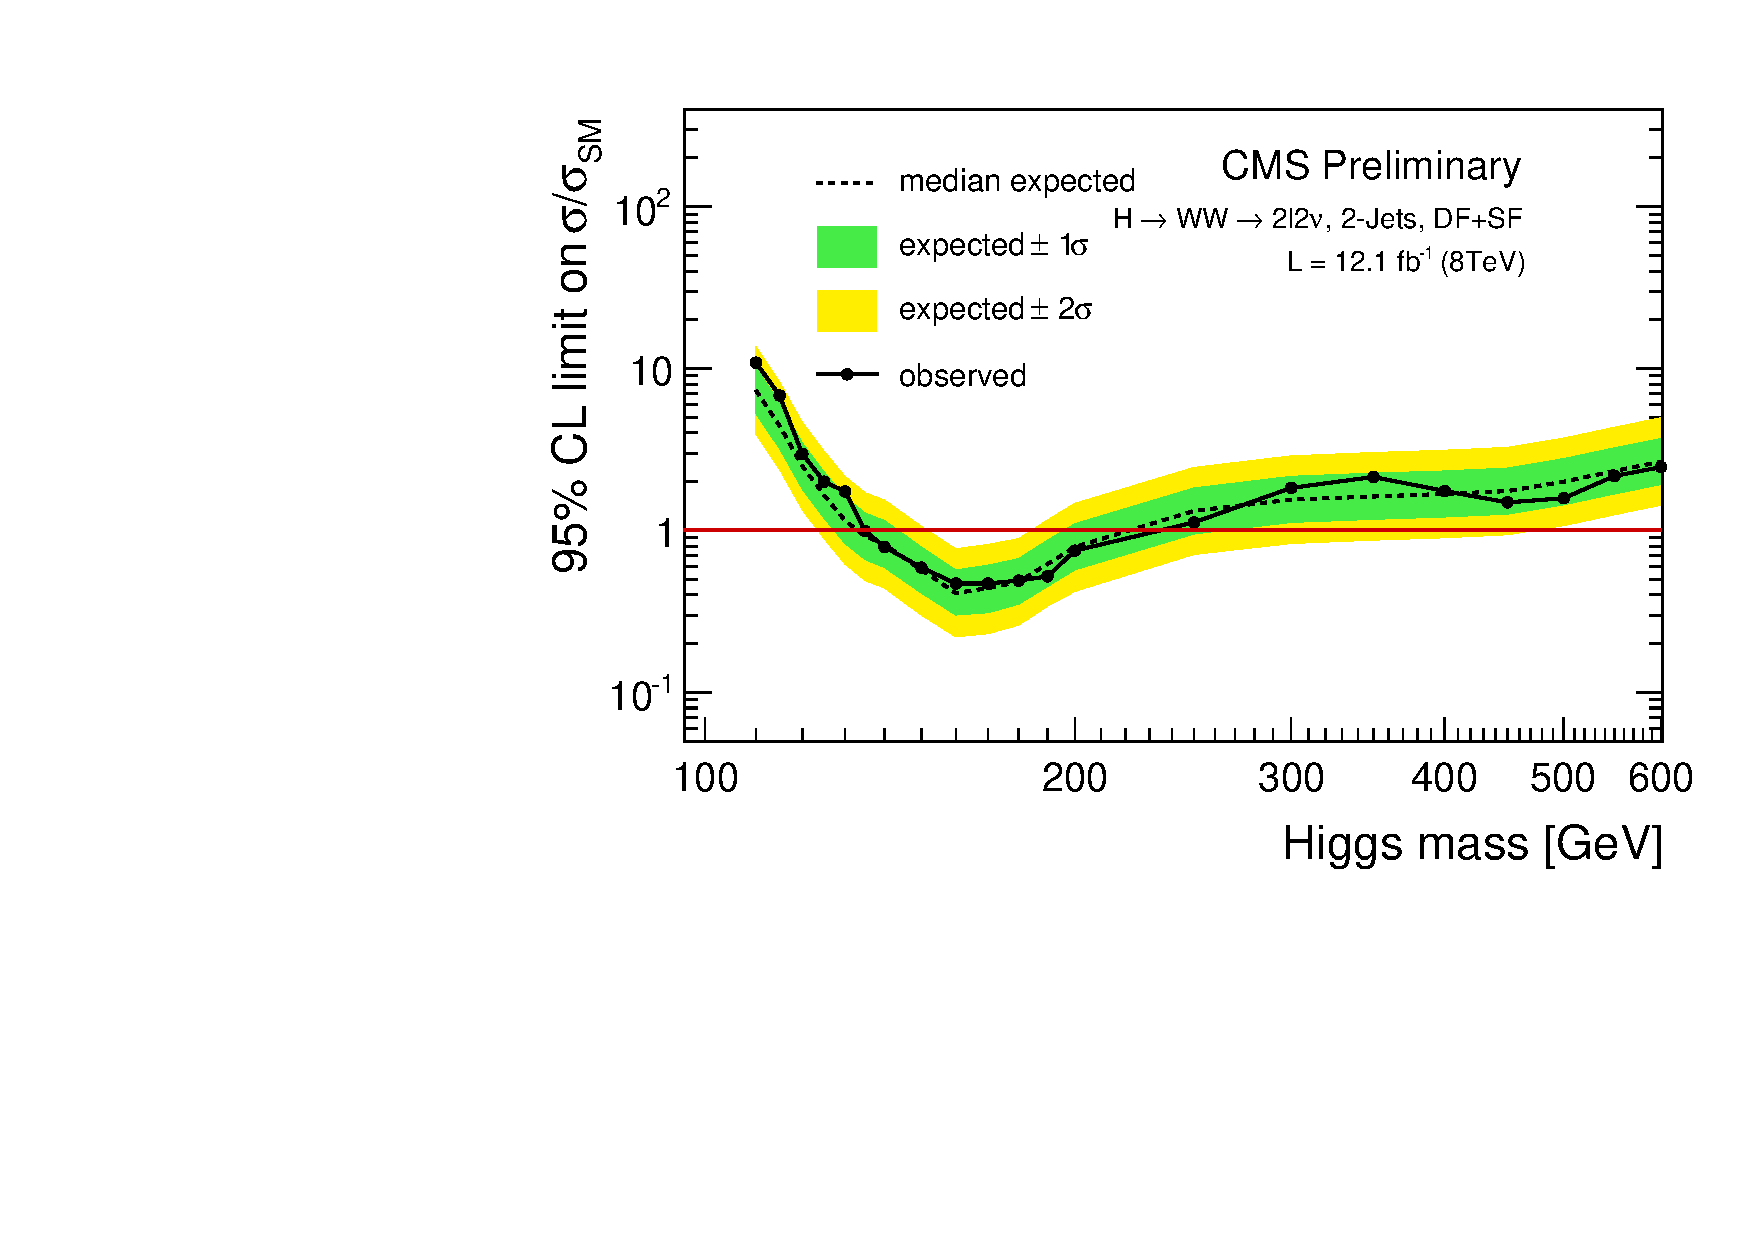
\includegraphics[width=.75\textwidth]{figures/table_limits_2j_cut_log.pdf}
\caption{Expected upper limits for SM Higgs in $\intlumiEightTeV$ at 8 TeV in the VBF channel.
The cut-based result is used. }
\label{fig:uls_2j_cut}
\end{figure}
% table
\begin{table}[!htbp]
\begin{center}
\begin{tabular}{c c c c c}
\hline
\vspace{-3mm} && \\
Higgs Mass & Observed  & Median expected & Expected range for 68\% & Expected range for 95\%   \\
\hline
110 & 10.88 & 7.33 & [5.28, 10.20] & [3.93, 13.67] \\
115 & 6.81 & 4.43 & [3.19, 6.17] & [2.38, 8.27] \\
120 & 2.97 & 2.50 & [1.80, 3.47] & [1.34, 4.65] \\
125 & 2.00 & 1.65 & [1.19, 2.30] & [0.89, 3.09] \\
130 & 1.74 & 1.15 & [0.83, 1.61] & [0.62, 2.15] \\
135 & 0.99 & 0.92 & [0.66, 1.28] & [0.49, 1.71] \\
140 & 0.79 & 0.82 & [0.59, 1.15] & [0.44, 1.54] \\
150 & 0.59 & 0.57 & [0.41, 0.79] & [0.30, 1.06] \\
160 & 0.47 & 0.41 & [0.30, 0.57] & [0.22, 0.77] \\
170 & 0.47 & 0.44 & [0.31, 0.61] & [0.23, 0.82] \\
180 & 0.49 & 0.48 & [0.35, 0.67] & [0.26, 0.89] \\
190 & 0.52 & 0.62 & [0.45, 0.87] & [0.34, 1.16] \\
200 & 0.75 & 0.79 & [0.57, 1.10] & [0.42, 1.47] \\
250 & 1.12 & 1.32 & [0.95, 1.83] & [0.71, 2.45] \\
300 & 1.83 & 1.55 & [1.12, 2.16] & [0.83, 2.89] \\
350 & 2.14 & 1.62 & [1.17, 2.26] & [0.87, 3.03] \\
400 & 1.75 & 1.68 & [1.21, 2.33] & [0.90, 3.13] \\
450 & 1.49 & 1.75 & [1.26, 2.43] & [0.94, 3.26] \\
500 & 1.58 & 2.00 & [1.44, 2.78] & [1.07, 3.72] \\
550 & 2.17 & 2.33 & [1.68, 3.24] & [1.25, 4.34] \\
600 & 2.46 & 2.66 & [1.92, 3.70] & [1.43, 4.97] \\
\vspace{-3mm} && \\
\hline
\end{tabular}
\caption{Expected upper limits for SM Higgs in $\intlumiEightTeV$ at 8 TeV in the VBF channel.
The cut-based result is used. }
\label{tab:uls_2j_cut}
\end{center}
\end{table}
%%%%%%%%%%

%%%%%%%%%%%%%%%%%
% plot
\begin{figure}[!hbtp]
\centering
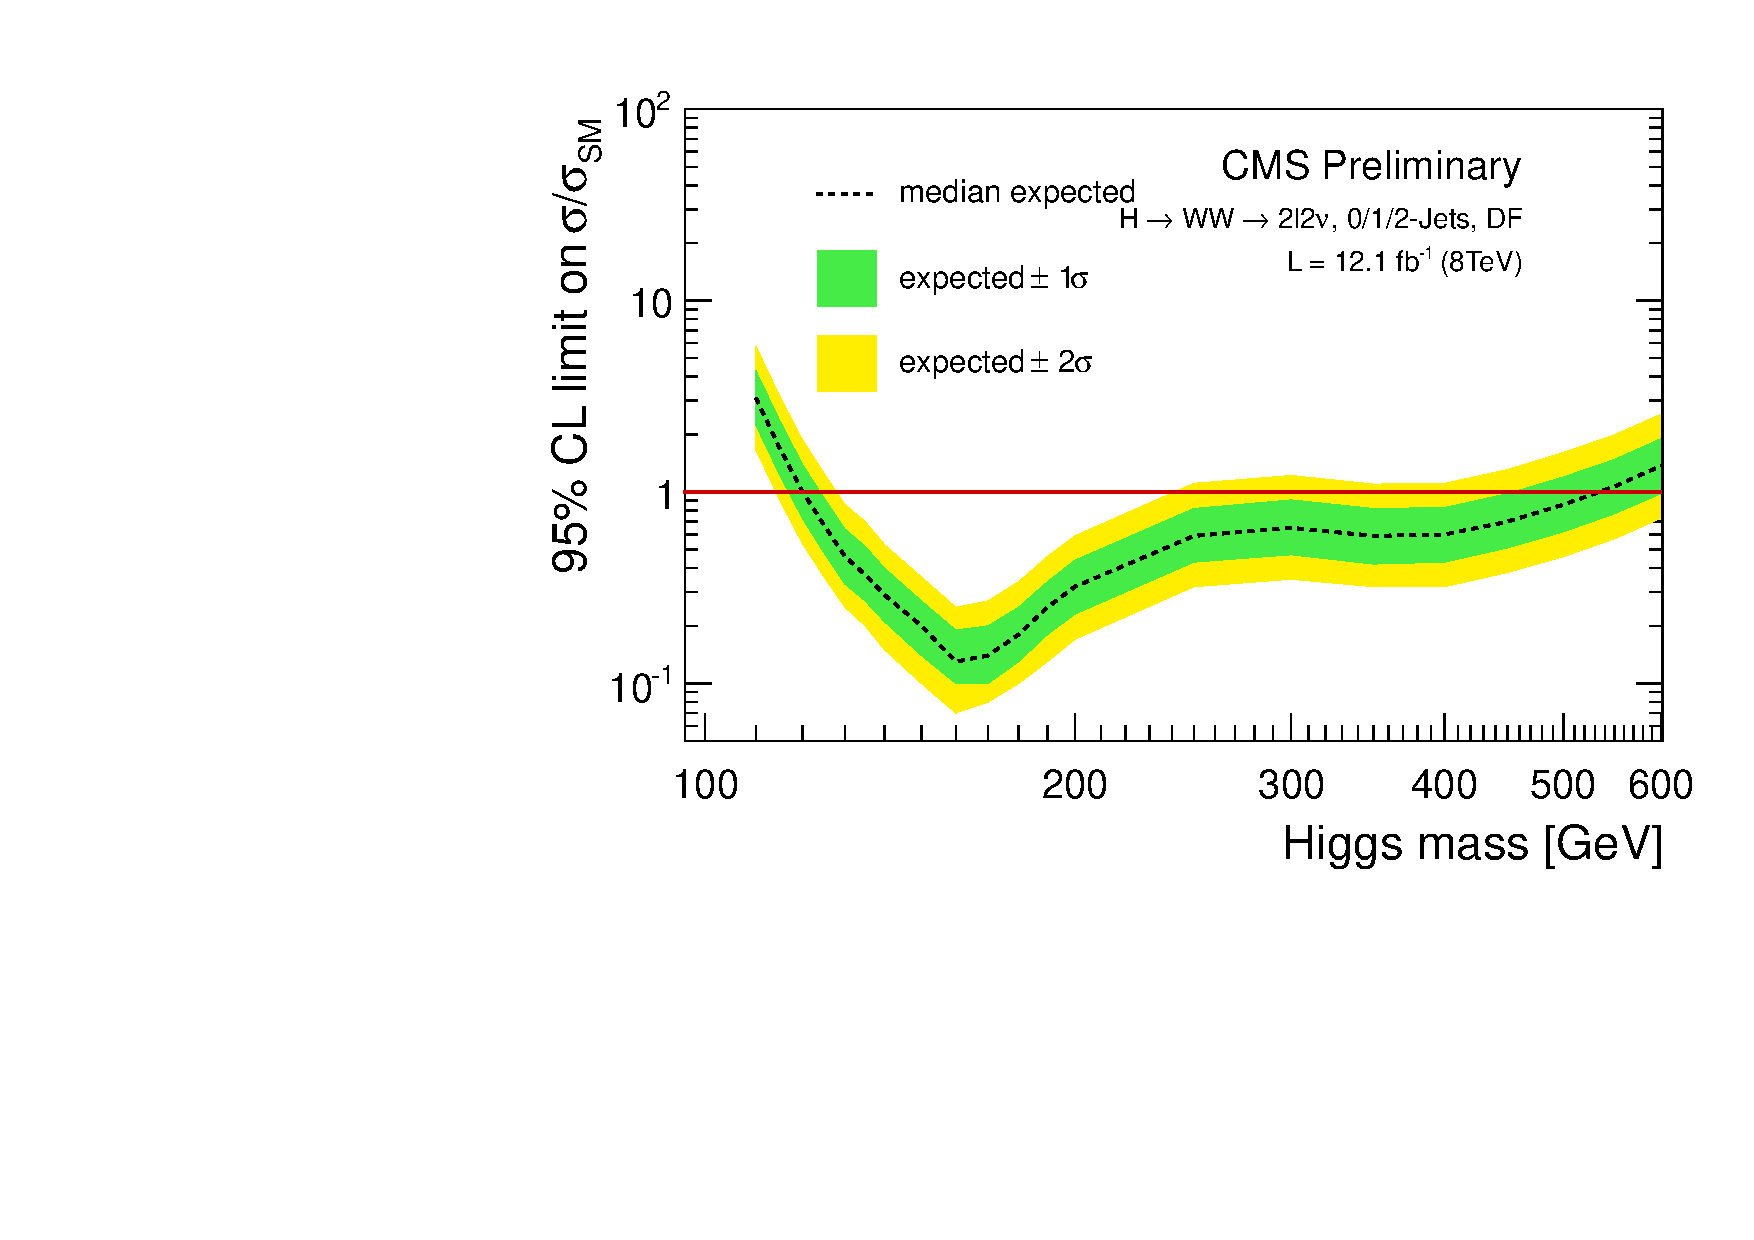
\includegraphics[width=.75\textwidth]{figures/table_limits_nj_shapebdt_of_cut_log.pdf}
\caption{Expected and observed upper limits for SM Higgs in $\intlumiEightTeV$ at 8 TeV in the $e\mu$ channel. 
BDT result is used for 0/1jet bin and cut-based result is used for VBF channel. }
\label{fig:uls_of_bdt01_cut2}
\end{figure}
% table
\begin{table}[!htbp]
\begin{center}
\begin{tabular}{c c c c c}
\hline
\vspace{-3mm} && \\
Higgs Mass & Observed  & Median expected & Expected range for 68\% & Expected range for 95\%   \\
\hline
\vspace{-3mm} && \\
110 & 5.27 & 3.29 & [2.37, 4.58] & [1.77, 6.14] \\
115 & 3.10 & 1.70 & [1.23, 2.37] & [0.91, 3.18] \\
120 & 1.62 & 1.01 & [0.73, 1.40] & [0.54, 1.88] \\
125 & 0.98 & 0.67 & [0.48, 0.93] & [0.36, 1.25] \\
130 & 0.73 & 0.46 & [0.33, 0.64] & [0.25, 0.86] \\
135 & 0.71 & 0.38 & [0.27, 0.52] & [0.20, 0.70] \\
140 & 0.54 & 0.29 & [0.21, 0.40] & [0.15, 0.54] \\
150 & 0.39 & 0.20 & [0.14, 0.27] & [0.10, 0.36] \\
160 & 0.19 & 0.13 & [0.10, 0.19] & [0.07, 0.25] \\
170 & 0.27 & 0.14 & [0.10, 0.20] & [0.08, 0.27] \\
180 & 0.39 & 0.18 & [0.13, 0.25] & [0.10, 0.34] \\
190 & 0.60 & 0.25 & [0.18, 0.34] & [0.13, 0.46] \\
200 & 0.79 & 0.32 & [0.23, 0.44] & [0.17, 0.59] \\
250 & 0.49 & 0.59 & [0.43, 0.83] & [0.32, 1.11] \\
300 & 0.49 & 0.65 & [0.47, 0.91] & [0.35, 1.22] \\
350 & 0.38 & 0.59 & [0.43, 0.82] & [0.32, 1.10] \\
400 & 0.36 & 0.60 & [0.43, 0.83] & [0.32, 1.11] \\
450 & 0.44 & 0.70 & [0.51, 0.98] & [0.38, 1.31] \\
500 & 0.54 & 0.86 & [0.62, 1.20] & [0.46, 1.61] \\
550 & 0.76 & 1.07 & [0.77, 1.48] & [0.57, 1.99] \\
600 & 0.97 & 1.37 & [0.99, 1.90] & [0.73, 2.55] \\
\hline
\end{tabular}
\caption{Expected and observed upper limits for SM Higgs in $\intlumiEightTeV$ at 8 TeV in the $e\mu$ channel. 
BDT result is used for 0/1jet bin and cut-based result is used for VBF channel. }
\label{tab:uls_of_bdt01_cut2}
\end{center}
\end{table} 
%%%%%%%%%%

%%%%%%%%%%%%%%%%%
% plot
\begin{figure}[!hbtp]
\centering
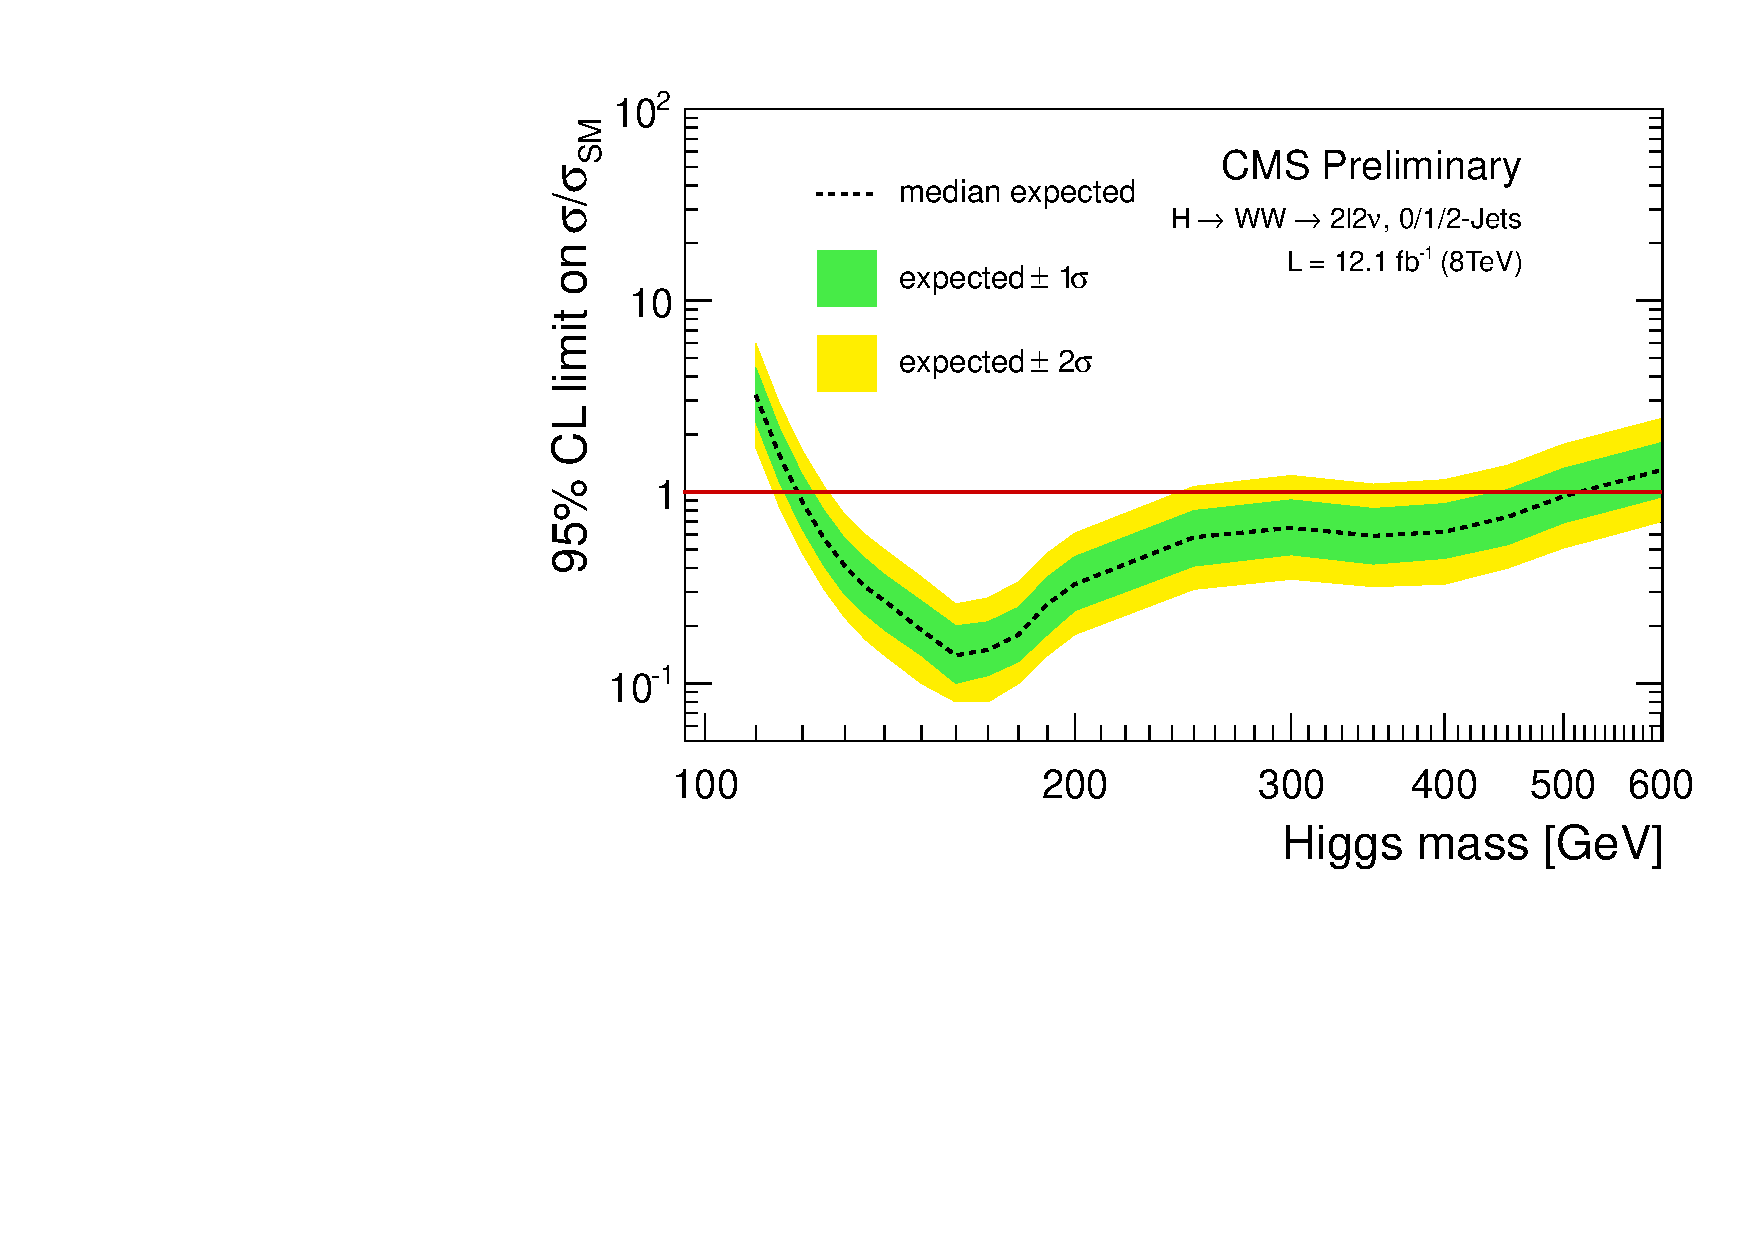
\includegraphics[width=.75\textwidth]{figures/table_limits_nj_shape2d_of_cut_log.pdf}
\caption{Expected and observed upper limits for SM Higgs in $\intlumiEightTeV$ at 8 TeV in the $e\mu$ channel. 
2D result is used for 0/1jet bin and cut-based result is used for VBF channel. }
\label{fig:uls_of_2d01_cut2}
\end{figure}
% table
\begin{table}[!htbp]
\begin{center}
\begin{tabular}{c c c c c}
\hline
\vspace{-3mm} && \\
Higgs Mass & Observed  & Median expected & Expected range for 68\% & Expected range for 95\%   \\
\hline
\vspace{-3mm} && \\
110 & 6.06 & 3.01 & [2.17, 4.19] & [1.61, 5.61] \\
115 & 3.23 & 1.55 & [1.11, 2.15] & [0.83, 2.88] \\
120 & 2.04 & 0.89 & [0.64, 1.25] & [0.48, 1.67] \\
125 & 1.21 & 0.58 & [0.42, 0.81] & [0.31, 1.08] \\
130 & 0.90 & 0.41 & [0.30, 0.58] & [0.22, 0.77] \\
135 & 0.71 & 0.33 & [0.24, 0.46] & [0.18, 0.61] \\
140 & 0.62 & 0.27 & [0.20, 0.38] & [0.15, 0.51] \\
150 & 0.41 & 0.20 & [0.15, 0.28] & [0.11, 0.38] \\
160 & 0.25 & 0.15 & [0.11, 0.21] & [0.08, 0.28] \\
170 & 0.25 & 0.16 & [0.12, 0.23] & [0.09, 0.30] \\
180 & 0.33 & 0.20 & [0.14, 0.28] & [0.11, 0.37] \\
190 & 0.46 & 0.28 & [0.20, 0.39] & [0.15, 0.52] \\
200 & 0.55 & 0.35 & [0.25, 0.49] & [0.19, 0.65] \\
250 & 0.56 & 0.60 & [0.43, 0.84] & [0.32, 1.13] \\
300 & 0.56 & 0.68 & [0.49, 0.95] & [0.37, 1.27] \\
350 & 0.42 & 0.61 & [0.44, 0.85] & [0.33, 1.13] \\
400 & 0.41 & 0.64 & [0.46, 0.90] & [0.35, 1.20] \\
450 & 0.52 & 0.82 & [0.59, 1.14] & [0.44, 1.52] \\
500 & 0.73 & 1.09 & [0.78, 1.51] & [0.58, 2.03] \\
550 & 1.17 & 1.36 & [0.98, 1.89] & [0.73, 2.54] \\
600 & 1.81 & 1.74 & [1.25, 2.42] & [0.93, 3.24] \\
\hline
\end{tabular}
\caption{Expected and observed upper limits for SM Higgs in $\intlumiEightTeV$ at 8 TeV in the $e\mu$ channel. 
2D result is used for 0/1jet bin and cut-based result is used for VBF channel. }
\label{tab:uls_of_2d01_cut2}
\end{center}
\end{table} 
%%%%%%%%%% 


%%%%%%%%%%%%%%%%%
% plot
\begin{figure}[!hbtp]
\centering
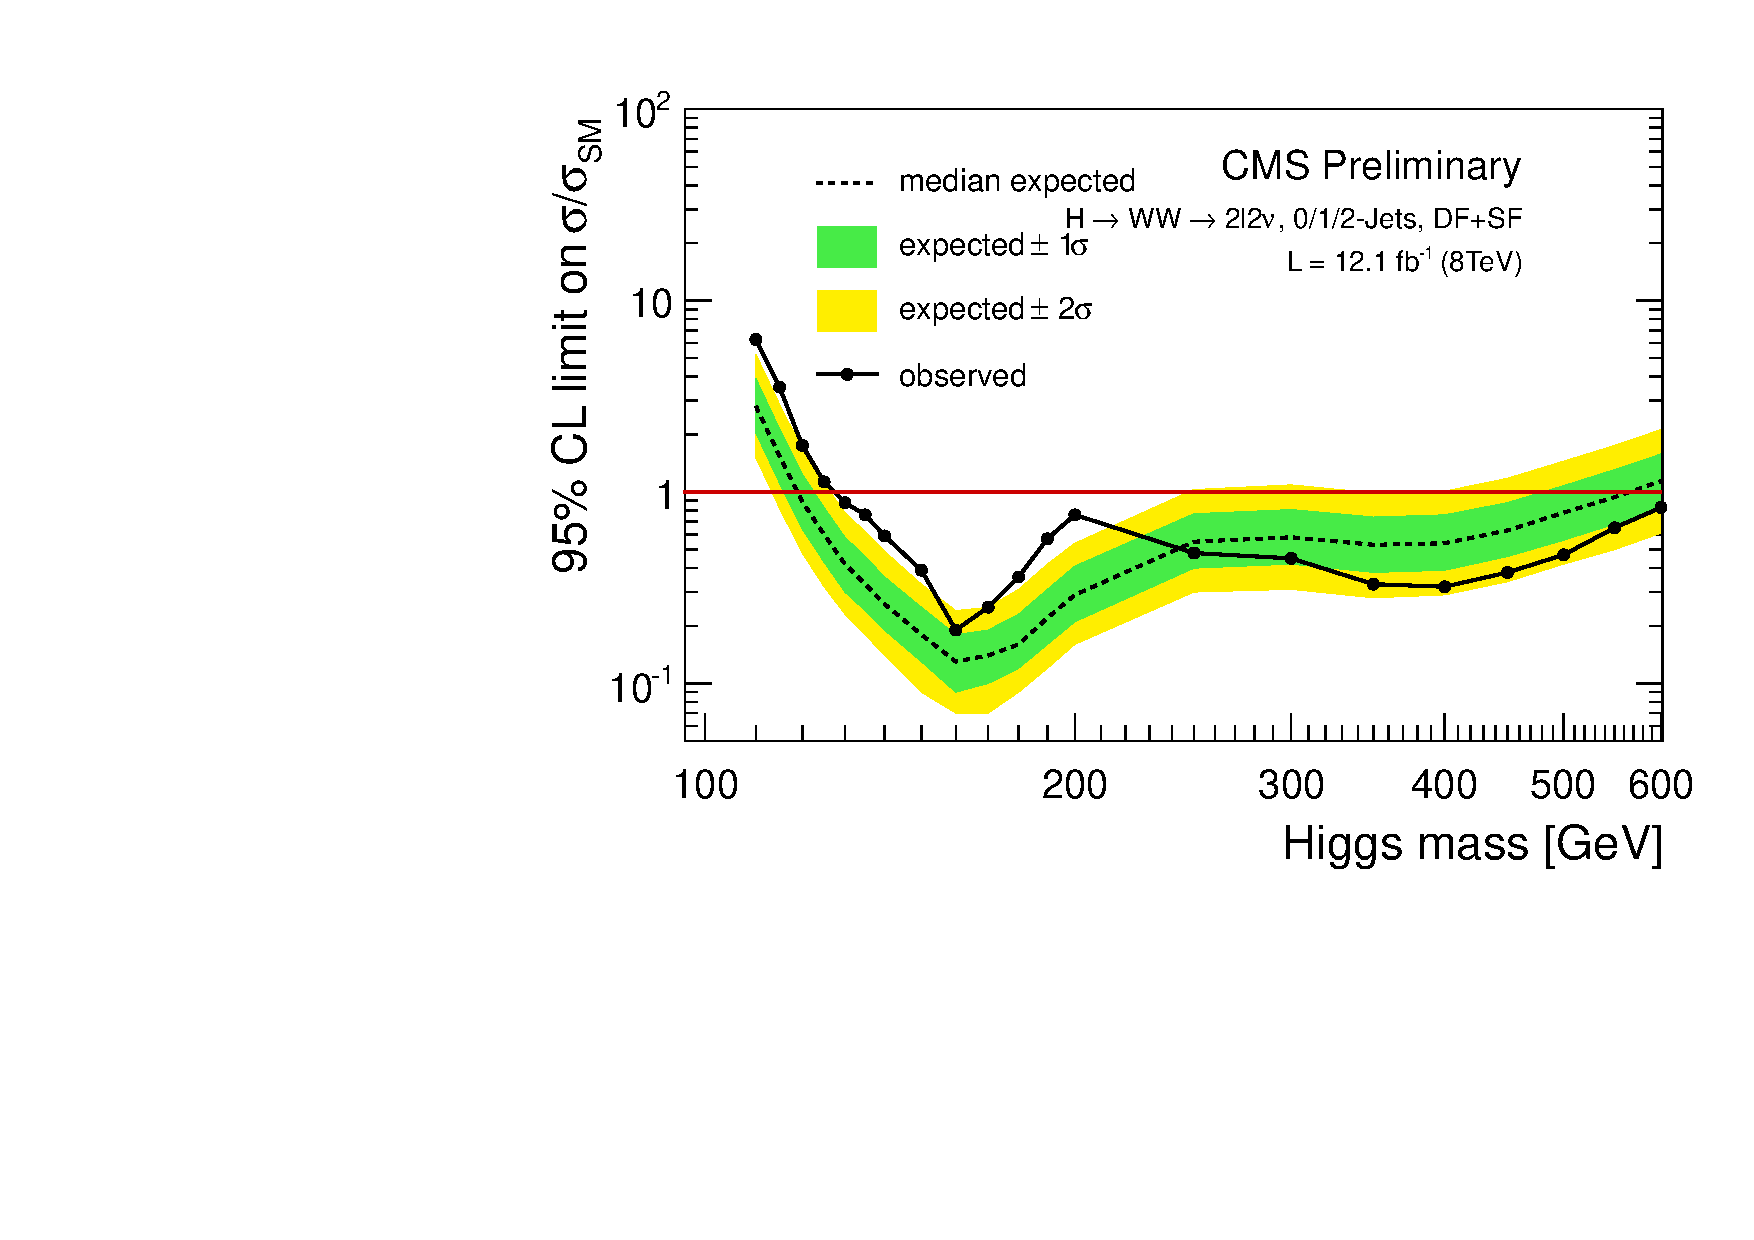
\includegraphics[width=.75\textwidth]{figures/table_limits_nj_shapebdt_of_cut_sf_log.pdf}
\caption{Expected upper limits for SM Higgs in $\intlumiEightTeV$ at 8 TeV.
BDT result is used for OF 0/1jet bin and cut-based result is used for VBF channel
and in the SF final states. }
\label{fig:uls_bdt01_cut2_cutsf}
\end{figure}
% table
\begin{table}[!htbp]
\begin{center}
\begin{tabular}{c c c c c}
\hline
\vspace{-3mm} && \\
Higgs Mass & Observed  & Median expected & Expected range for 68\% & Expected range for 95\%   \\
\hline
110 & 6.26 & 2.81 & [2.03, 3.92] & [1.51, 5.25] \\
115 & 3.53 & 1.54 & [1.11, 2.14] & [0.82, 2.87] \\
120 & 1.75 & 0.89 & [0.64, 1.24] & [0.48, 1.67] \\
125 & 1.13 & 0.60 & [0.43, 0.83] & [0.32, 1.11] \\
130 & 0.88 & 0.42 & [0.30, 0.58] & [0.23, 0.78] \\
135 & 0.76 & 0.33 & [0.24, 0.46] & [0.18, 0.62] \\
140 & 0.59 & 0.26 & [0.19, 0.36] & [0.14, 0.49] \\
150 & 0.39 & 0.18 & [0.13, 0.25] & [0.09, 0.33] \\
160 & 0.19 & 0.13 & [0.09, 0.18] & [0.07, 0.24] \\
170 & 0.25 & 0.14 & [0.10, 0.19] & [0.07, 0.25] \\
180 & 0.36 & 0.16 & [0.12, 0.23] & [0.09, 0.31] \\
190 & 0.57 & 0.22 & [0.16, 0.31] & [0.12, 0.42] \\
200 & 0.76 & 0.29 & [0.21, 0.41] & [0.16, 0.54] \\
250 & 0.48 & 0.55 & [0.40, 0.77] & [0.30, 1.03] \\
300 & 0.45 & 0.58 & [0.42, 0.81] & [0.31, 1.09] \\
350 & 0.33 & 0.53 & [0.38, 0.74] & [0.28, 0.99] \\
400 & 0.32 & 0.54 & [0.39, 0.76] & [0.29, 1.01] \\
450 & 0.38 & 0.63 & [0.46, 0.88] & [0.34, 1.18] \\
500 & 0.47 & 0.78 & [0.56, 1.08] & [0.42, 1.45] \\
550 & 0.65 & 0.94 & [0.68, 1.31] & [0.50, 1.75] \\
600 & 0.83 & 1.14 & [0.82, 1.58] & [0.61, 2.12] \\
\vspace{-3mm} && \\
\hline
\end{tabular}
\caption{Expected upper limits for SM Higgs in $\intlumiEightTeV$ at 8 TeV.
BDT result is used for OF 0/1jet bin and cut-based result is used for VBF channel
and in the SF final states. }
\label{tab:uls_bdt01_cut2_cutsf}
\end{center}
\end{table}
%%%%%%%%%%

%%%%%%%%%%%%%%%%%
% plot
\begin{figure}[!hbtp]
\centering
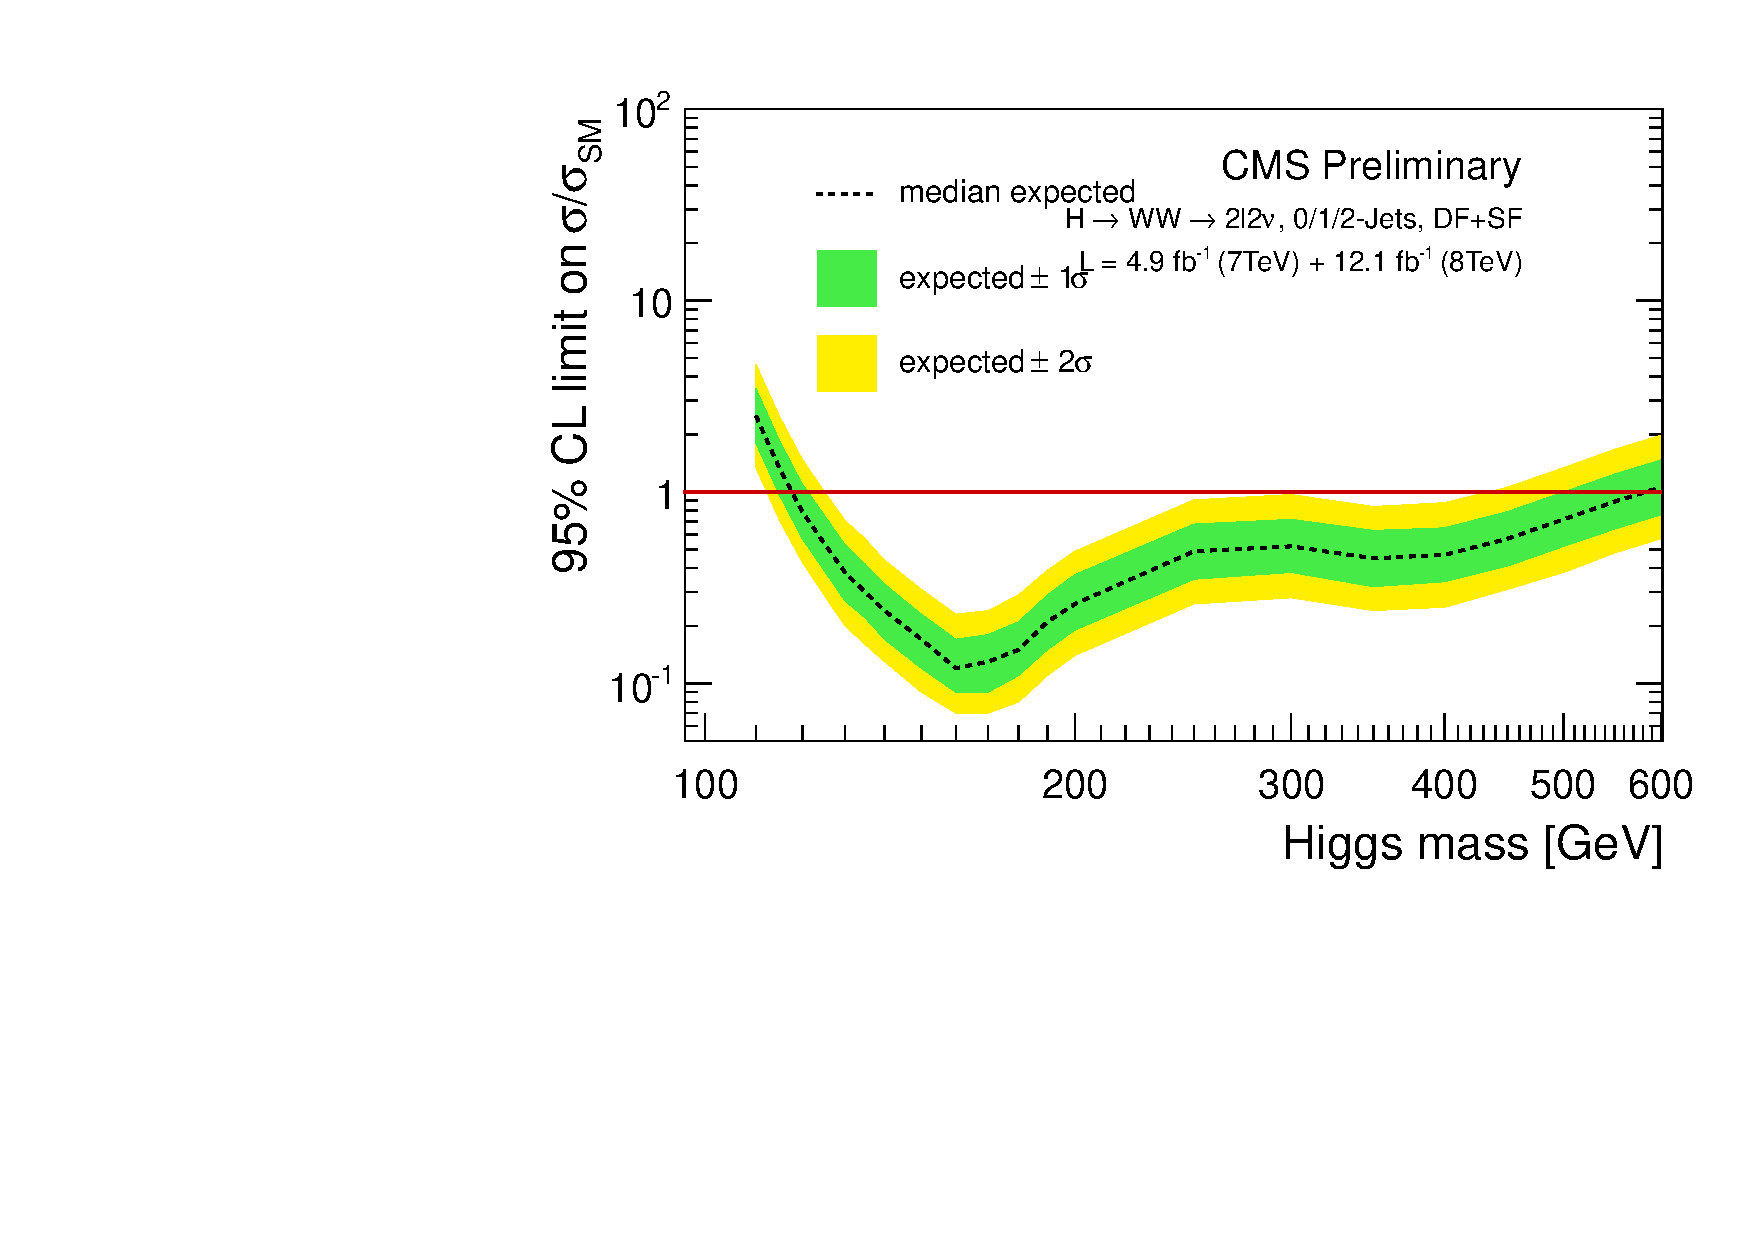
\includegraphics[width=.75\textwidth]{figures/table_limits_nj_8TeV_shapebdt_of_cut_7TeV_shape_log.pdf}
\caption{Expected and observed upper limits for SM Higgs combining the $\intlumiSevenTeV$ data
at 7 TeV and the $\intlumiEightTeV$ at 8 TeV.
For the 0 and 1 Jet bin final states, the 7 TeV analysis uses the shape based approach for all
lepton flavor final states, while the 8 TeV analysis uses the BDT based approach 
in the $e\mu$ channel in 0/1jet bins and cut-based approch $e\mu$ 2jets and same flavor final states.}
\label{fig:uls_bdt01_cut2_cutsf_comb}
\end{figure}
% table
\begin{table}[!htbp]
\begin{center}
\begin{tabular}{c c c c c}
\hline
\vspace{-3mm} && \\
Higgs Mass & Observed  & Median expected & Expected range for 68\% & Expected range for 95\%   \\
\hline
110 & 6.17 & 2.45 & [1.77, 3.41] & [1.32, 4.57] \\
115 & 3.27 & 1.31 & [0.94, 1.82] & [0.70, 2.44] \\
120 & 1.78 & 0.78 & [0.56, 1.08] & [0.42, 1.45] \\
125 & 1.09 & 0.53 & [0.38, 0.73] & [0.28, 0.98] \\
130 & 0.84 & 0.37 & [0.26, 0.51] & [0.20, 0.69] \\
135 & 0.70 & 0.29 & [0.21, 0.40] & [0.16, 0.54] \\
140 & 0.55 & 0.23 & [0.17, 0.32] & [0.12, 0.43] \\
150 & 0.37 & 0.16 & [0.12, 0.23] & [0.09, 0.31] \\
160 & 0.19 & 0.12 & [0.09, 0.17] & [0.07, 0.23] \\
170 & 0.23 & 0.13 & [0.09, 0.18] & [0.07, 0.24] \\
180 & 0.28 & 0.15 & [0.11, 0.21] & [0.08, 0.29] \\
190 & 0.42 & 0.21 & [0.15, 0.29] & [0.11, 0.39] \\
200 & 0.55 & 0.26 & [0.19, 0.37] & [0.14, 0.49] \\
250 & 0.40 & 0.49 & [0.35, 0.68] & [0.26, 0.91] \\
300 & 0.42 & 0.52 & [0.37, 0.72] & [0.28, 0.97] \\
350 & 0.31 & 0.45 & [0.32, 0.63] & [0.24, 0.84] \\
400 & 0.31 & 0.47 & [0.34, 0.65] & [0.25, 0.88] \\
450 & 0.35 & 0.57 & [0.41, 0.79] & [0.31, 1.06] \\
500 & 0.43 & 0.72 & [0.52, 1.00] & [0.38, 1.34] \\
550 & 0.61 & 0.89 & [0.64, 1.24] & [0.48, 1.67] \\
600 & 0.73 & 1.06 & [0.76, 1.47] & [0.57, 1.98] \\
\vspace{-3mm} && \\
\hline
\end{tabular}
\caption{Expected and observed upper limits for SM Higgs combining the $\intlumiSevenTeV$ data
at 7 TeV and the $\intlumiEightTeV$ at 8 TeV.
For the 0 and 1 Jet bin final states, the 7 TeV analysis uses the shape based approach for all
lepton flavor final states, while the 8 TeV analysis uses the BDT based approach 
in the $e\mu$ channel in 0/1jet bins and cut-based approch $e\mu$ 2jets and same flavor final states.}
\label{tab:uls_bdt01_cut2_cutsf_comb}
\end{center}
\end{table} 
%%%%%%%%%%



%%%%%%%%%%%%%%%%%%%%%%%%%%%%%%%%%%
%%%%    Individual channels  %%%%%
%%%%%%%%%%%%%%%%%%%%%%%%%%%%%%%%%%

\newpage
%%%%%%%%%%%%%%%%%
% plot
\begin{figure}[!hbtp]
\centering
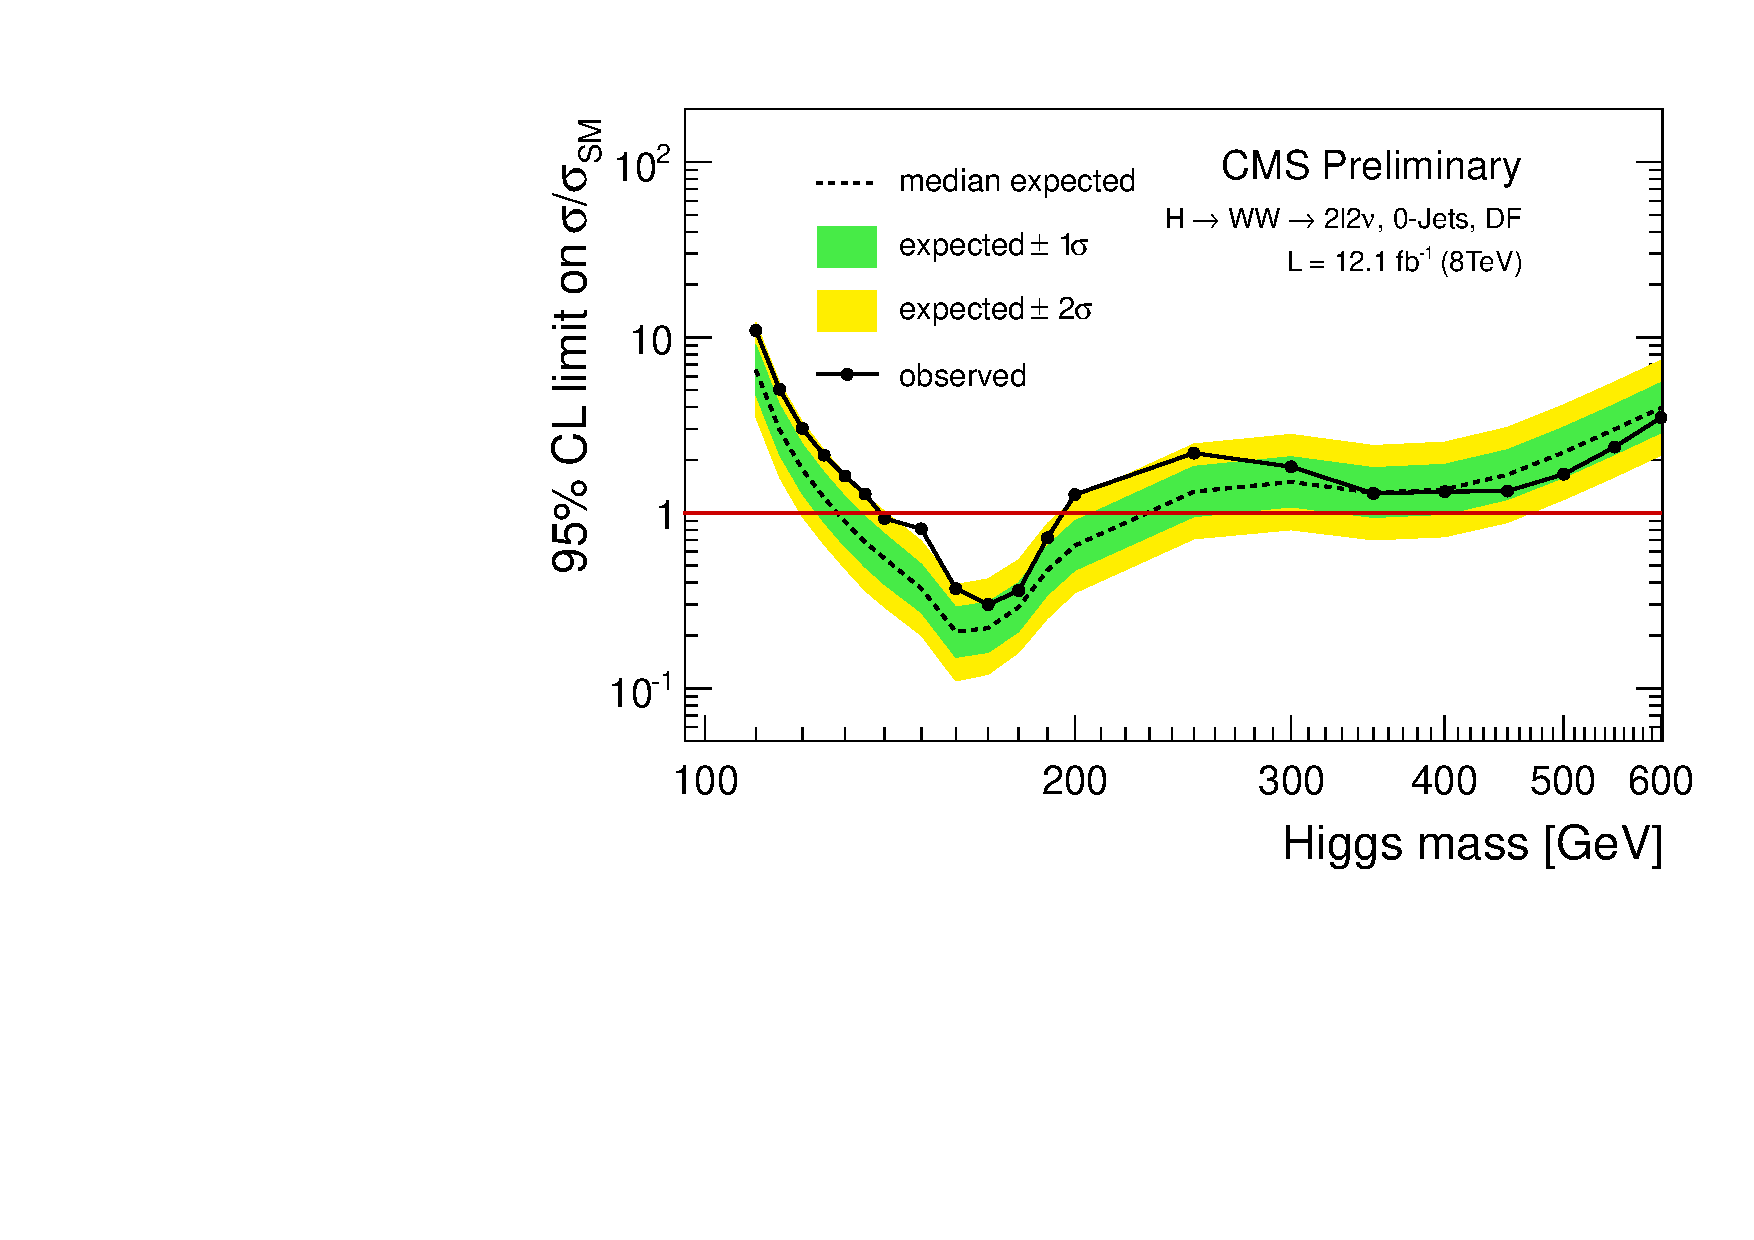
\includegraphics[width=.75\textwidth]{figures/table_limits_0j_cut_of_log.pdf}
\caption{Expected upper limits for SM Higgs in $\intlumiEightTeV$ at 8 TeV with cut-based analysis in 0jet bin in DF final states.}
\label{fig:uls_cut_0j_of}
\end{figure}
% table
\begin{table}[!htbp]
\begin{center}
\begin{tabular}{c c c c c}
\hline
\vspace{-3mm} && \\
Higgs Mass & Observed  & Median expected & Expected range for 68\% & Expected range for 95\%   \\
\hline
110 & 10.94 & 6.52 & [4.69, 9.07] & [3.50, 12.16] \\
115 & 5.06 & 2.97 & [2.14, 4.13] & [1.59, 5.54] \\
120 & 3.03 & 1.77 & [1.28, 2.47] & [0.95, 3.30] \\
125 & 2.13 & 1.22 & [0.88, 1.70] & [0.66, 2.28] \\
130 & 1.62 & 0.89 & [0.64, 1.24] & [0.48, 1.67] \\
135 & 1.28 & 0.68 & [0.49, 0.95] & [0.36, 1.27] \\
140 & 0.93 & 0.55 & [0.39, 0.76] & [0.29, 1.02] \\
150 & 0.81 & 0.37 & [0.27, 0.51] & [0.20, 0.69] \\
160 & 0.37 & 0.21 & [0.15, 0.29] & [0.11, 0.39] \\
170 & 0.30 & 0.22 & [0.16, 0.31] & [0.12, 0.42] \\
180 & 0.36 & 0.29 & [0.21, 0.40] & [0.16, 0.54] \\
190 & 0.72 & 0.47 & [0.34, 0.65] & [0.25, 0.87] \\
200 & 1.27 & 0.65 & [0.47, 0.90] & [0.35, 1.21] \\
250 & 2.19 & 1.32 & [0.95, 1.84] & [0.71, 2.47] \\
300 & 1.83 & 1.50 & [1.08, 2.09] & [0.80, 2.80] \\
350 & 1.29 & 1.30 & [0.94, 1.81] & [0.70, 2.42] \\
400 & 1.32 & 1.36 & [0.98, 1.89] & [0.73, 2.53] \\
450 & 1.33 & 1.65 & [1.19, 2.29] & [0.88, 3.07] \\
500 & 1.66 & 2.21 & [1.59, 3.08] & [1.19, 4.13] \\
550 & 2.37 & 2.99 & [2.15, 4.15] & [1.60, 5.57] \\
600 & 3.49 & 3.97 & [2.86, 5.53] & [2.13, 7.41] \\
\vspace{-3mm} && \\
\hline
\end{tabular}
\caption{Expected upper limits for SM Higgs in $\intlumiEightTeV$ at 8 TeV with cut-based analysis in 0jet bin in DF final states.}
\label{tab:uls_cut_0j_of}
\end{center}
\end{table}
%%%%%%%%%%

%%%%%%%%%%%%%%%%%
% plot
\begin{figure}[!hbtp]
\centering
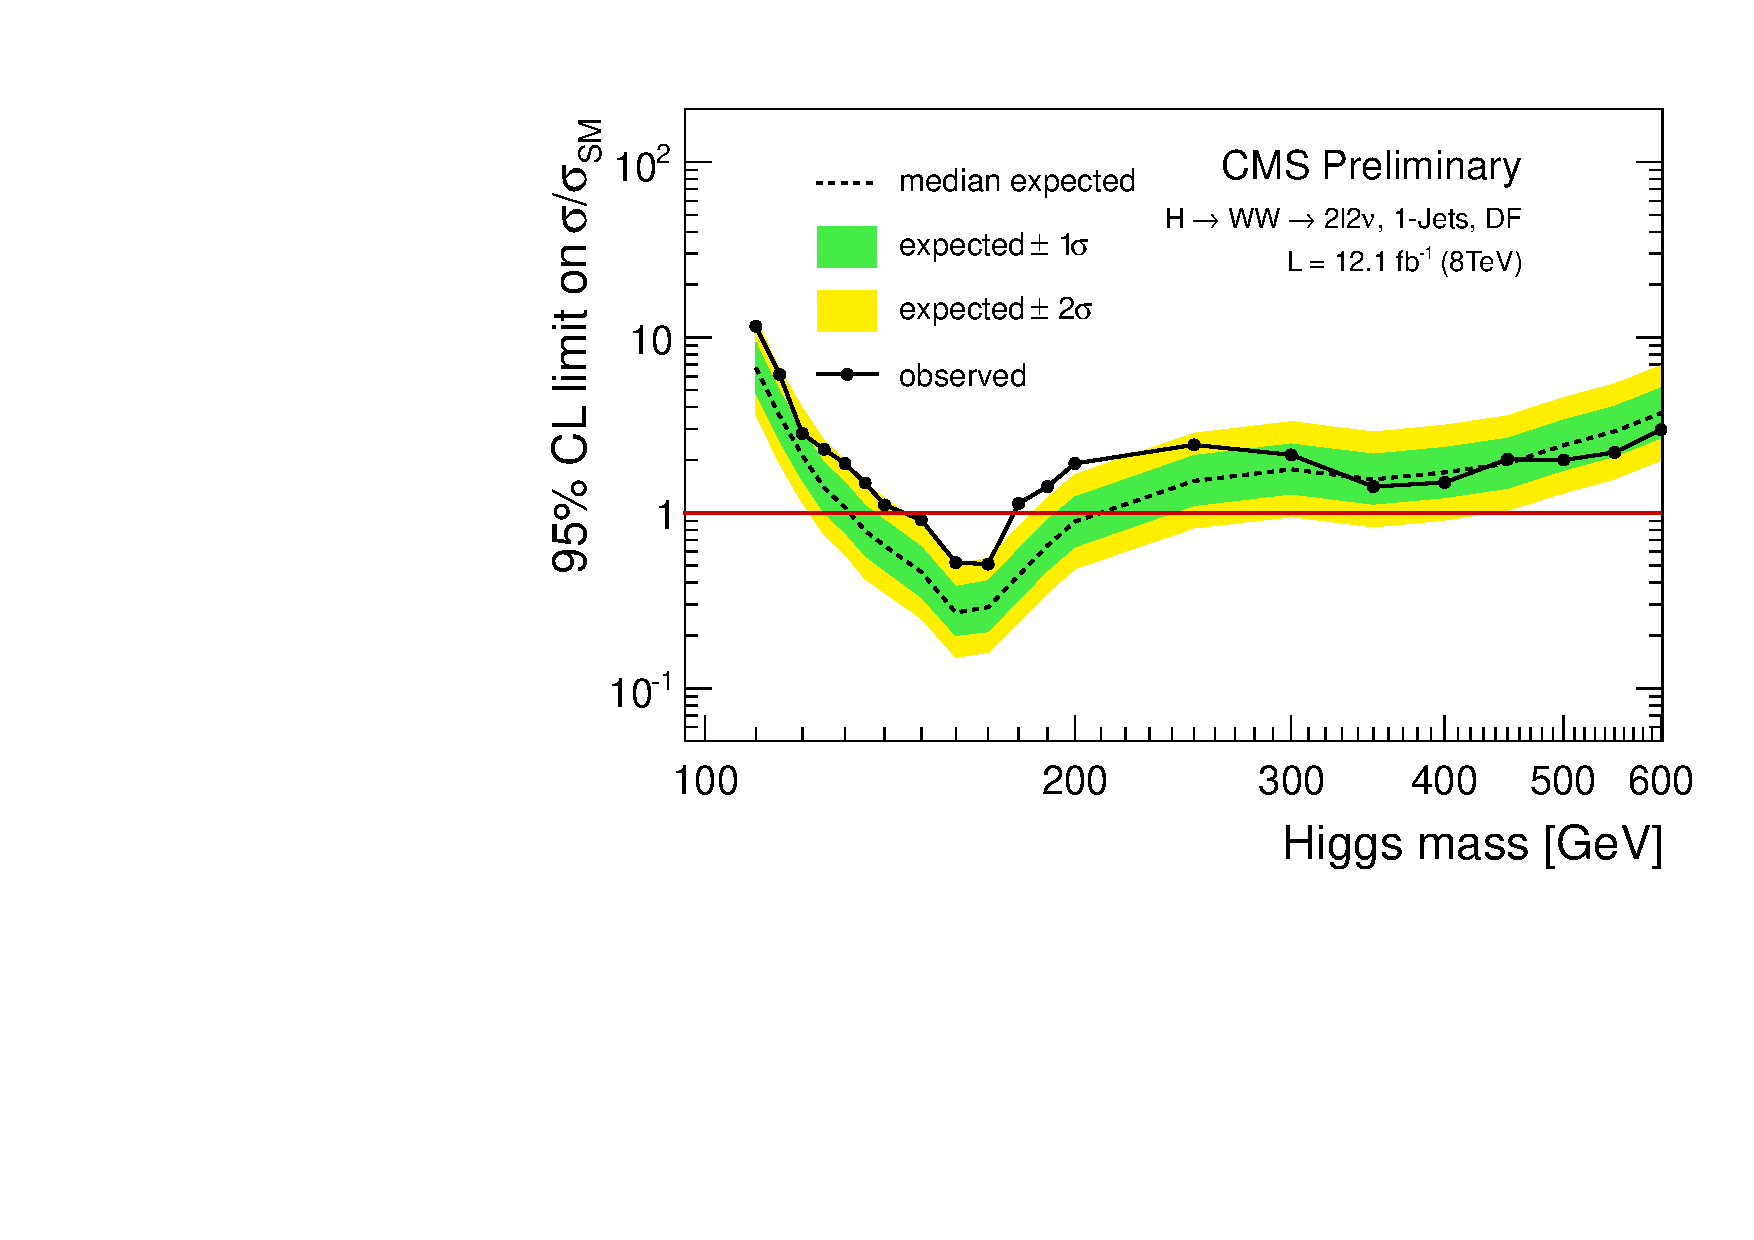
\includegraphics[width=.75\textwidth]{figures/table_limits_1j_cut_of_log.pdf}
\caption{Expected upper limits for SM Higgs in $\intlumiEightTeV$ at 8 TeV with cut-based analysis in 1jet bin in DF final states.}
\label{fig:uls_cut_1j_of}
\end{figure}
% table
\begin{table}[!htbp]
\begin{center}
\begin{tabular}{c c c c c}
\hline
\vspace{-3mm} && \\
Higgs Mass & Observed  & Median expected & Expected range for 68\% & Expected range for 95\%   \\
\hline
110 & 11.57 & 6.71 & [4.83, 9.33] & [3.60, 12.51] \\
115 & 6.15 & 3.57 & [2.57, 4.96] & [1.91, 6.65] \\
120 & 2.83 & 2.12 & [1.53, 2.95] & [1.14, 3.96] \\
125 & 2.30 & 1.39 & [1.00, 1.93] & [0.75, 2.59] \\
130 & 1.91 & 1.07 & [0.77, 1.49] & [0.58, 2.00] \\
135 & 1.48 & 0.79 & [0.57, 1.10] & [0.42, 1.47] \\
140 & 1.11 & 0.65 & [0.47, 0.91] & [0.35, 1.22] \\
150 & 0.91 & 0.46 & [0.33, 0.64] & [0.25, 0.86] \\
160 & 0.52 & 0.27 & [0.20, 0.38] & [0.15, 0.51] \\
170 & 0.51 & 0.29 & [0.21, 0.41] & [0.16, 0.55] \\
180 & 1.13 & 0.44 & [0.32, 0.62] & [0.24, 0.83] \\
190 & 1.41 & 0.65 & [0.47, 0.91] & [0.35, 1.22] \\
200 & 1.91 & 0.89 & [0.64, 1.23] & [0.48, 1.65] \\
250 & 2.44 & 1.52 & [1.10, 2.12] & [0.82, 2.84] \\
300 & 2.14 & 1.77 & [1.28, 2.47] & [0.95, 3.31] \\
350 & 1.41 & 1.55 & [1.12, 2.16] & [0.83, 2.89] \\
400 & 1.49 & 1.70 & [1.22, 2.36] & [0.91, 3.16] \\
450 & 2.02 & 1.91 & [1.38, 2.66] & [1.03, 3.57] \\
500 & 2.00 & 2.43 & [1.75, 3.38] & [1.30, 4.54] \\
550 & 2.21 & 2.91 & [2.10, 4.05] & [1.56, 5.43] \\
600 & 2.98 & 3.70 & [2.67, 5.15] & [1.99, 6.90] \\
\vspace{-3mm} && \\
\hline
\end{tabular}
\caption{Expected upper limits for SM Higgs in $\intlumiEightTeV$ at 8 TeV with cut-based analysis in 1jet bin in DF final states.}
\label{tab:uls_cut_1j_of}
\end{center}
\end{table}
%%%%%%%%%%

%%%%%%%%%%%%%%%%%
% plot
\begin{figure}[!hbtp]
\centering
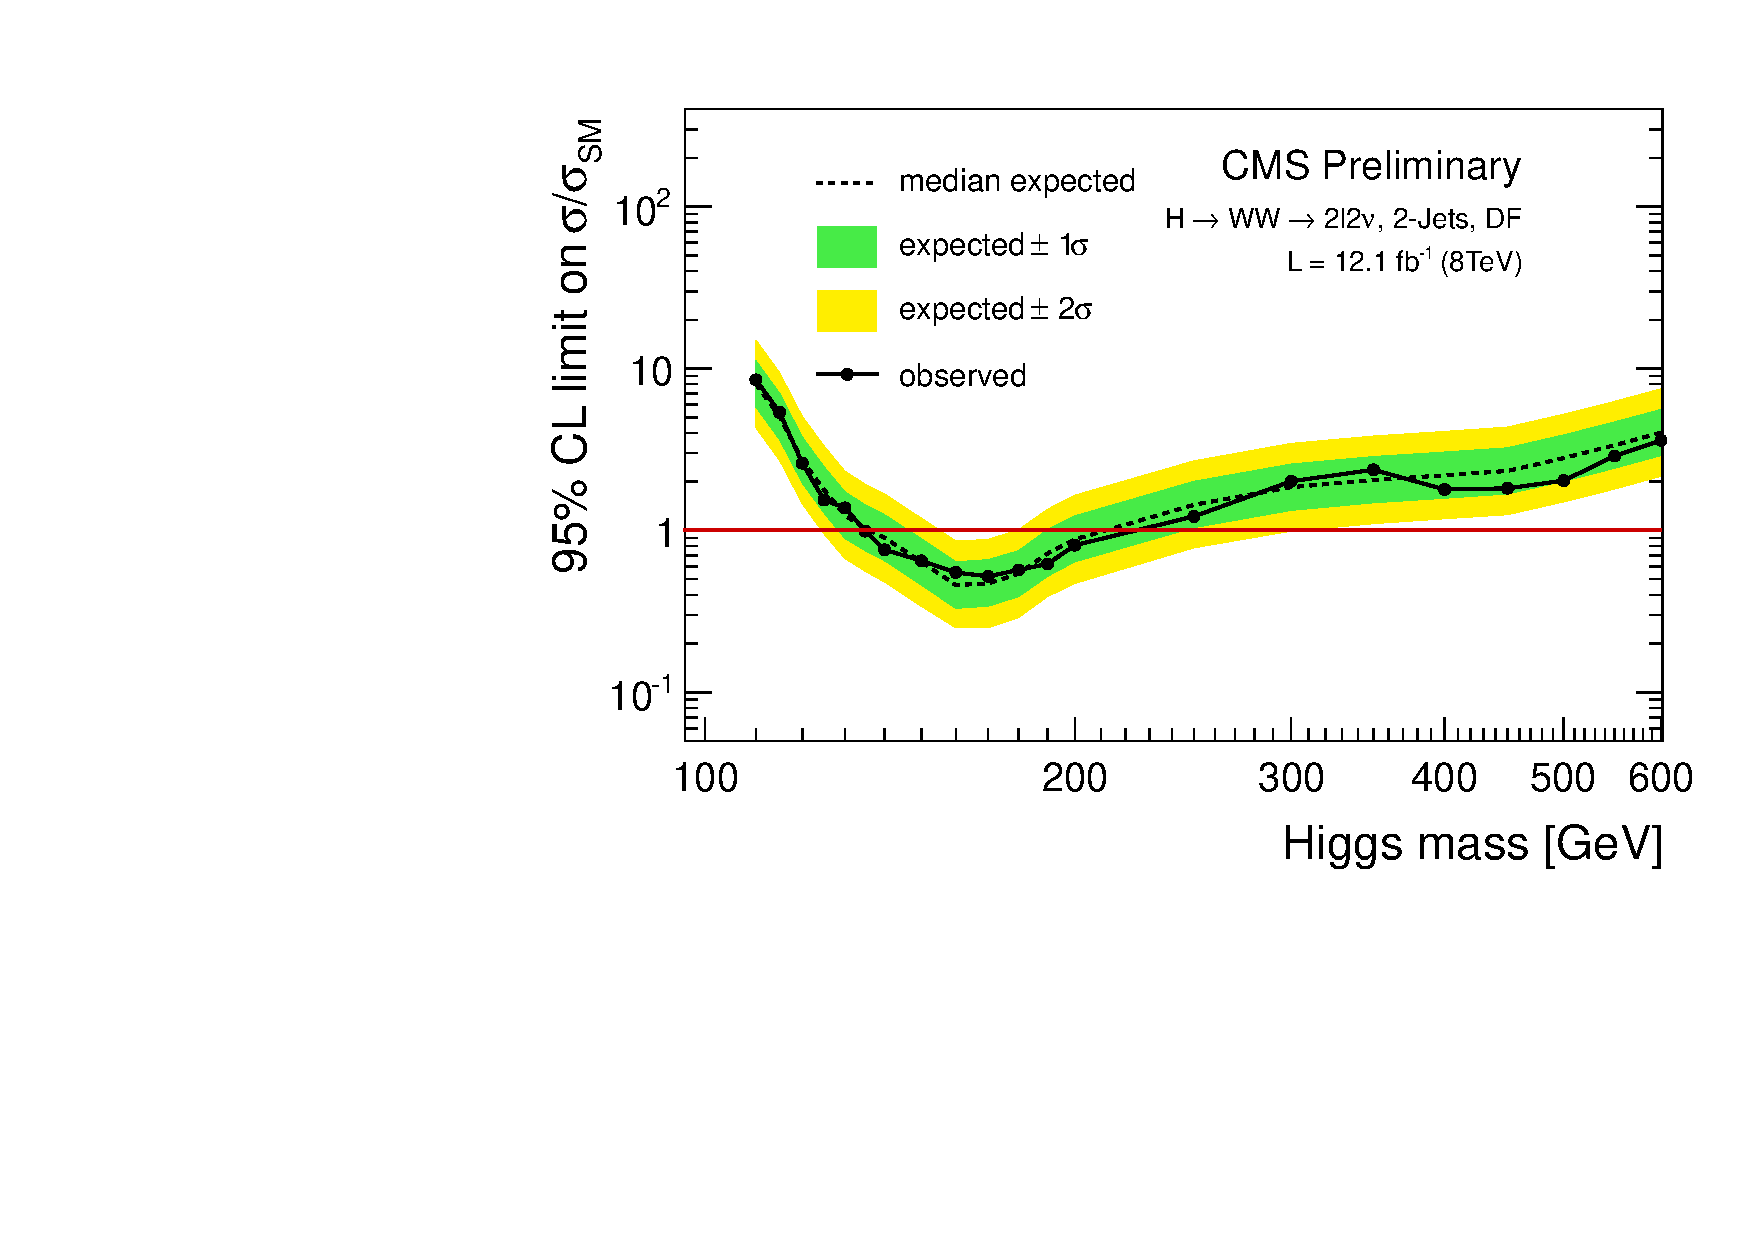
\includegraphics[width=.75\textwidth]{figures/table_limits_2j_cut_of_log.pdf}
\caption{Expected upper limits for SM Higgs in $\intlumiEightTeV$ at 8 TeV with cut-based analysis in 2jet bin in DF final states.}
\label{fig:uls_cut_2j_of}
\end{figure}
% table
\begin{table}[!htbp]
\begin{center}
\begin{tabular}{c c c c c}
\hline
\vspace{-3mm} && \\
Higgs Mass & Observed  & Median expected & Expected range for 68\% & Expected range for 95\%   \\
\hline
110 & 8.52 & 8.04 & [5.79, 11.19] & [4.31, 14.99] \\
115 & 5.36 & 5.06 & [3.64, 7.04] & [2.71, 9.43] \\
120 & 2.60 & 2.71 & [1.96, 3.78] & [1.46, 5.06] \\
125 & 1.54 & 1.78 & [1.28, 2.47] & [0.95, 3.32] \\
130 & 1.38 & 1.24 & [0.89, 1.73] & [0.67, 2.32] \\
135 & 0.99 & 1.03 & [0.75, 1.44] & [0.56, 1.93] \\
140 & 0.76 & 0.90 & [0.65, 1.25] & [0.48, 1.68] \\
150 & 0.65 & 0.64 & [0.46, 0.89] & [0.34, 1.19] \\
160 & 0.55 & 0.46 & [0.33, 0.64] & [0.25, 0.86] \\
170 & 0.52 & 0.47 & [0.34, 0.66] & [0.25, 0.88] \\
180 & 0.57 & 0.54 & [0.39, 0.75] & [0.29, 1.01] \\
190 & 0.62 & 0.72 & [0.52, 1.01] & [0.39, 1.35] \\
200 & 0.81 & 0.88 & [0.64, 1.23] & [0.47, 1.65] \\
250 & 1.22 & 1.44 & [1.04, 2.01] & [0.78, 2.69] \\
300 & 2.01 & 1.85 & [1.33, 2.57] & [0.99, 3.45] \\
350 & 2.37 & 2.05 & [1.48, 2.86] & [1.10, 3.83] \\
400 & 1.79 & 2.19 & [1.58, 3.05] & [1.18, 4.09] \\
450 & 1.82 & 2.33 & [1.68, 3.24] & [1.25, 4.35] \\
500 & 2.03 & 2.80 & [2.01, 3.89] & [1.50, 5.22] \\
550 & 2.88 & 3.36 & [2.42, 4.68] & [1.80, 6.27] \\
600 & 3.60 & 4.02 & [2.90, 5.59] & [2.16, 7.50] \\
\vspace{-3mm} && \\
\hline
\end{tabular}
\caption{Expected upper limits for SM Higgs in $\intlumiEightTeV$ at 8 TeV with cut-based analysis in 2jet bin in DF final states.}
\label{tab:uls_cut_2j_of}
\end{center}
\end{table}
%%%%%%%%%%

\newpage
%%%%%%%%%%%%%%%%%
% plot
\begin{figure}[!hbtp]
\centering
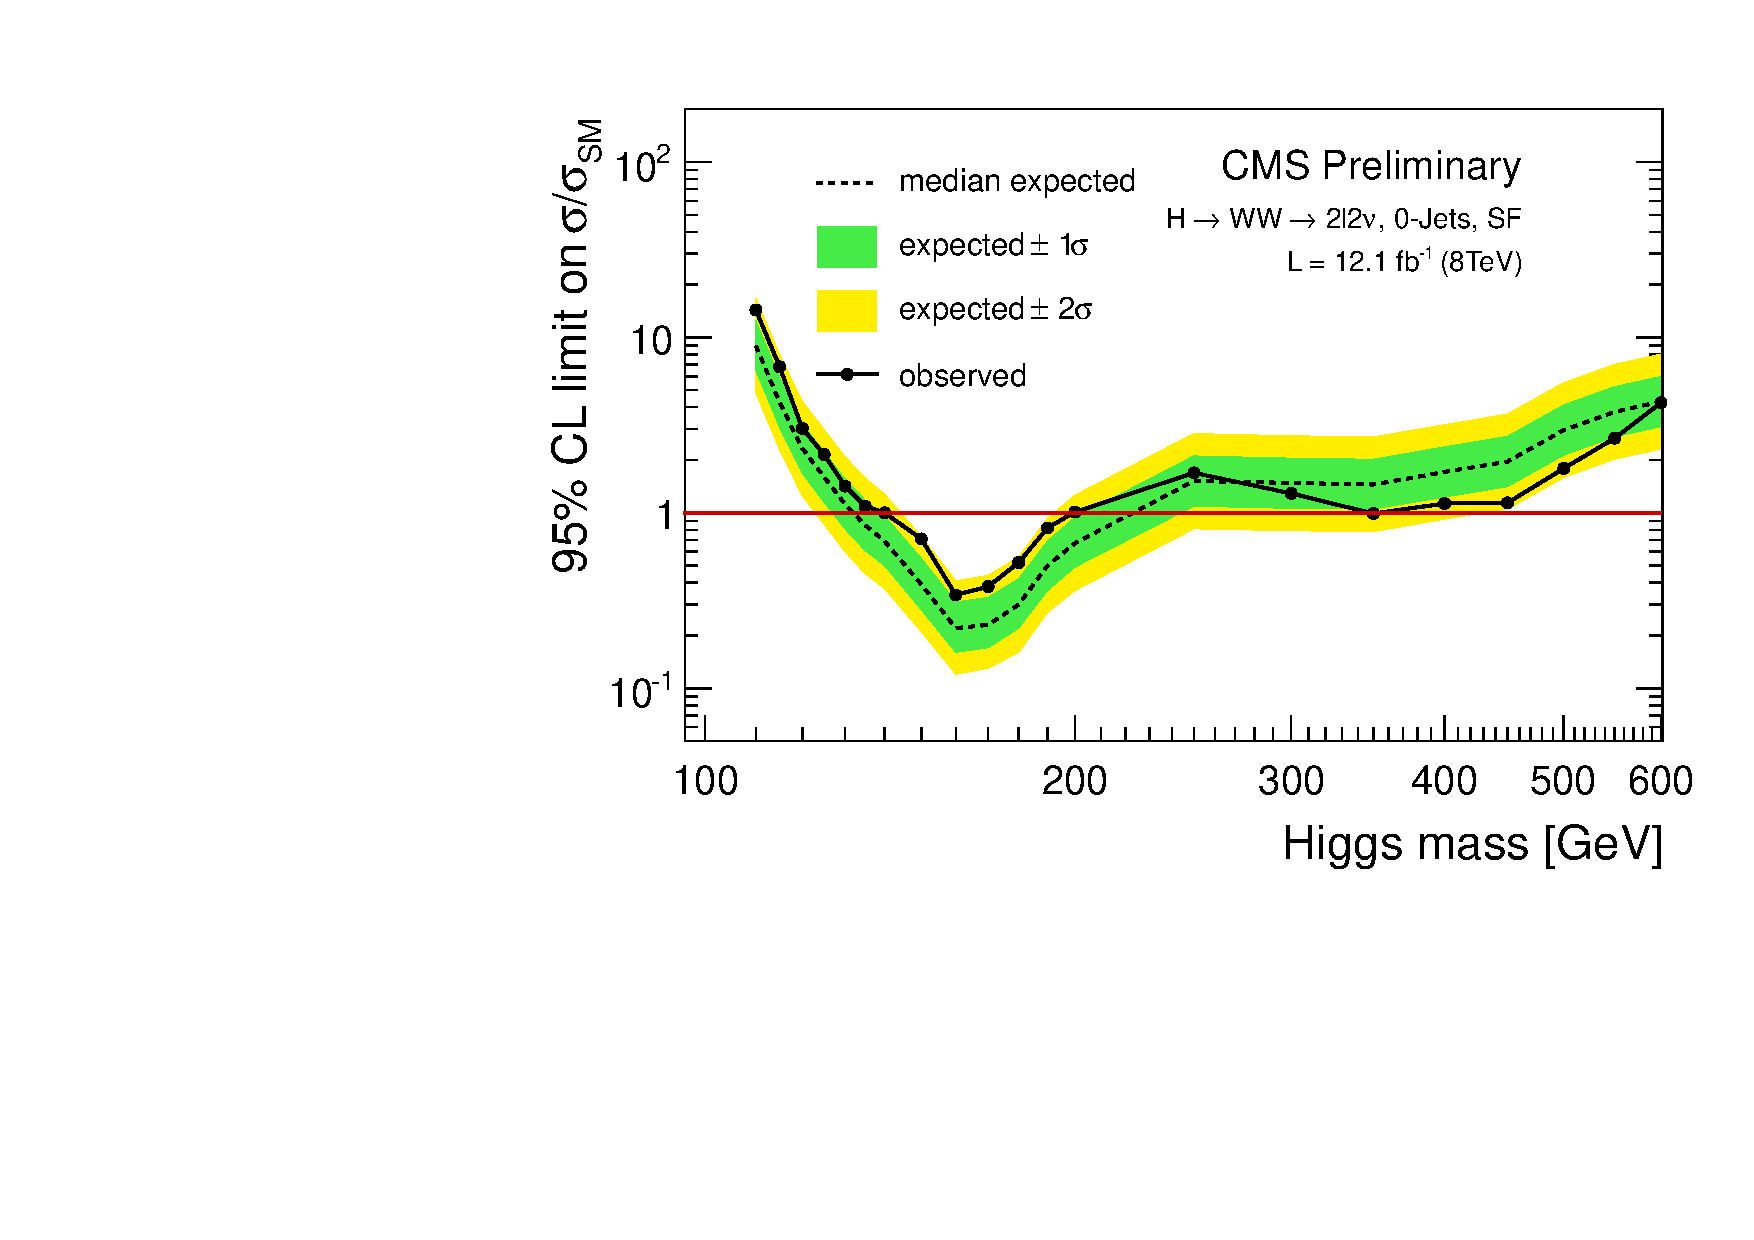
\includegraphics[width=.75\textwidth]{figures/table_limits_0j_cut_sf_log.pdf}
\caption{Expected upper limits for SM Higgs in $\intlumiEightTeV$ at 8 TeV with cut-based analysis in 0jet bin in sf final states.}
\label{fig:uls_cut_0j_sf}
\end{figure}
% table
\begin{table}[!htbp]
\begin{center}
\begin{tabular}{c c c c c}
\hline
\vspace{-3mm} && \\
Higgs Mass & Observed  & Median expected & Expected range for 68\% & Expected range for 95\%   \\
\hline
110 & 14.33 & 8.97 & [6.46, 12.48] & [4.81, 16.72] \\
115 & 6.80 & 4.26 & [3.07, 5.93] & [2.29, 7.95] \\
120 & 3.03 & 2.33 & [1.68, 3.24] & [1.25, 4.34] \\
125 & 2.15 & 1.60 & [1.15, 2.22] & [0.86, 2.98] \\
130 & 1.42 & 1.12 & [0.81, 1.56] & [0.60, 2.09] \\
135 & 1.09 & 0.85 & [0.61, 1.18] & [0.45, 1.58] \\
140 & 1.00 & 0.69 & [0.50, 0.96] & [0.37, 1.28] \\
150 & 0.71 & 0.39 & [0.28, 0.55] & [0.21, 0.73] \\
160 & 0.34 & 0.22 & [0.16, 0.31] & [0.12, 0.41] \\
170 & 0.38 & 0.23 & [0.17, 0.33] & [0.13, 0.44] \\
180 & 0.52 & 0.30 & [0.22, 0.42] & [0.16, 0.56] \\
190 & 0.82 & 0.50 & [0.36, 0.69] & [0.27, 0.93] \\
200 & 1.01 & 0.67 & [0.49, 0.94] & [0.36, 1.26] \\
250 & 1.69 & 1.52 & [1.09, 2.11] & [0.81, 2.83] \\
300 & 1.29 & 1.48 & [1.06, 2.05] & [0.79, 2.75] \\
350 & 0.99 & 1.45 & [1.05, 2.02] & [0.78, 2.71] \\
400 & 1.13 & 1.71 & [1.23, 2.38] & [0.92, 3.18] \\
450 & 1.14 & 1.96 & [1.41, 2.73] & [1.05, 3.66] \\
500 & 1.79 & 2.96 & [2.13, 4.12] & [1.59, 5.52] \\
550 & 2.66 & 3.76 & [2.71, 5.24] & [2.02, 7.02] \\
600 & 4.24 & 4.31 & [3.10, 5.99] & [2.31, 8.03] \\
\vspace{-3mm} && \\
\hline
\end{tabular}
\caption{Expected upper limits for SM Higgs in $\intlumiEightTeV$ at 8 TeV with cut-based analysis in 0jet bin in sf final states.}
\label{tab:uls_cut_0j_sf}
\end{center}
\end{table}
%%%%%%%%%%

%%%%%%%%%%%%%%%%%
% plot
\begin{figure}[!hbtp]
\centering
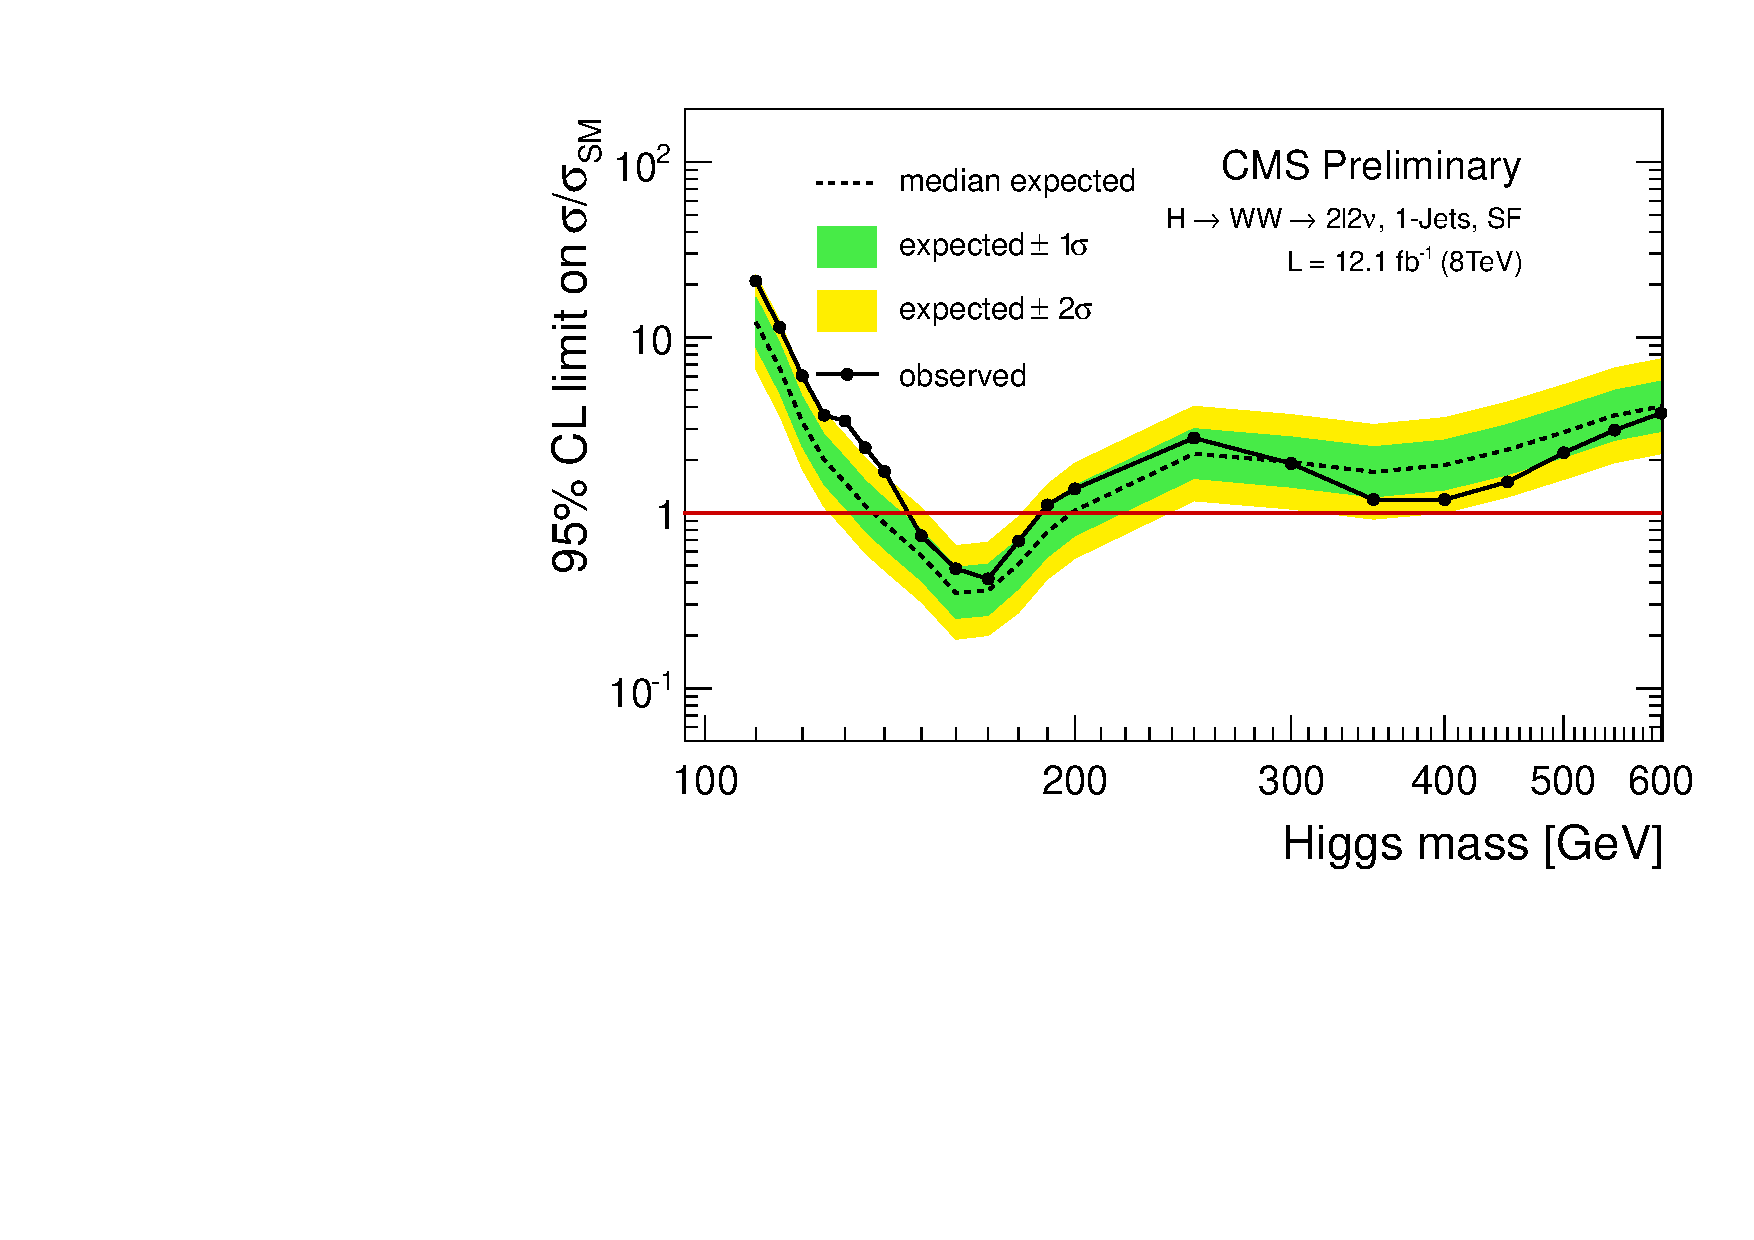
\includegraphics[width=.75\textwidth]{figures/table_limits_1j_cut_sf_log.pdf}
\caption{Expected upper limits for SM Higgs in $\intlumiEightTeV$ at 8 TeV with cut-based analysis in 1jet bin in sf final states.}
\label{fig:uls_cut_1j_sf}
\end{figure}
% table
\begin{table}[!htbp]
\begin{center}
\begin{tabular}{c c c c c}
\hline
\vspace{-3mm} && \\
Higgs Mass & Observed  & Median expected & Expected range for 68\% & Expected range for 95\%   \\
\hline
110 & 20.95 & 12.19 & [8.79, 16.97] & [6.54, 22.75] \\
115 & 11.43 & 6.70 & [4.83, 9.32] & [3.60, 12.50] \\
120 & 6.05 & 3.30 & [2.38, 4.59] & [1.77, 6.15] \\
125 & 3.60 & 2.01 & [1.45, 2.80] & [1.08, 3.76] \\
130 & 3.34 & 1.49 & [1.07, 2.07] & [0.80, 2.78] \\
135 & 2.35 & 1.10 & [0.79, 1.53] & [0.59, 2.05] \\
140 & 1.72 & 0.87 & [0.62, 1.21] & [0.47, 1.62] \\
150 & 0.74 & 0.57 & [0.41, 0.80] & [0.31, 1.07] \\
160 & 0.48 & 0.35 & [0.25, 0.49] & [0.19, 0.65] \\
170 & 0.42 & 0.36 & [0.26, 0.51] & [0.20, 0.68] \\
180 & 0.69 & 0.51 & [0.37, 0.71] & [0.27, 0.95] \\
190 & 1.11 & 0.78 & [0.56, 1.08] & [0.42, 1.45] \\
200 & 1.37 & 1.03 & [0.74, 1.43] & [0.55, 1.92] \\
250 & 2.67 & 2.17 & [1.57, 3.02] & [1.17, 4.05] \\
300 & 1.91 & 1.95 & [1.40, 2.71] & [1.05, 3.63] \\
350 & 1.19 & 1.71 & [1.23, 2.38] & [0.92, 3.19] \\
400 & 1.19 & 1.87 & [1.35, 2.60] & [1.00, 3.49] \\
450 & 1.50 & 2.29 & [1.65, 3.19] & [1.23, 4.28] \\
500 & 2.20 & 2.88 & [2.07, 4.01] & [1.55, 5.37] \\
550 & 2.96 & 3.59 & [2.59, 5.00] & [1.93, 6.70] \\
600 & 3.70 & 4.04 & [2.91, 5.63] & [2.17, 7.54] \\
\vspace{-3mm} && \\
\hline
\end{tabular}
\caption{Expected upper limits for SM Higgs in $\intlumiEightTeV$ at 8 TeV with cut-based analysis in 1jet bin in sf final states.}
\label{tab:uls_cut_1j_sf}
\end{center}
\end{table}
%%%%%%%%%%

%%%%%%%%%%%%%%%%%
% plot
\begin{figure}[!hbtp]
\centering
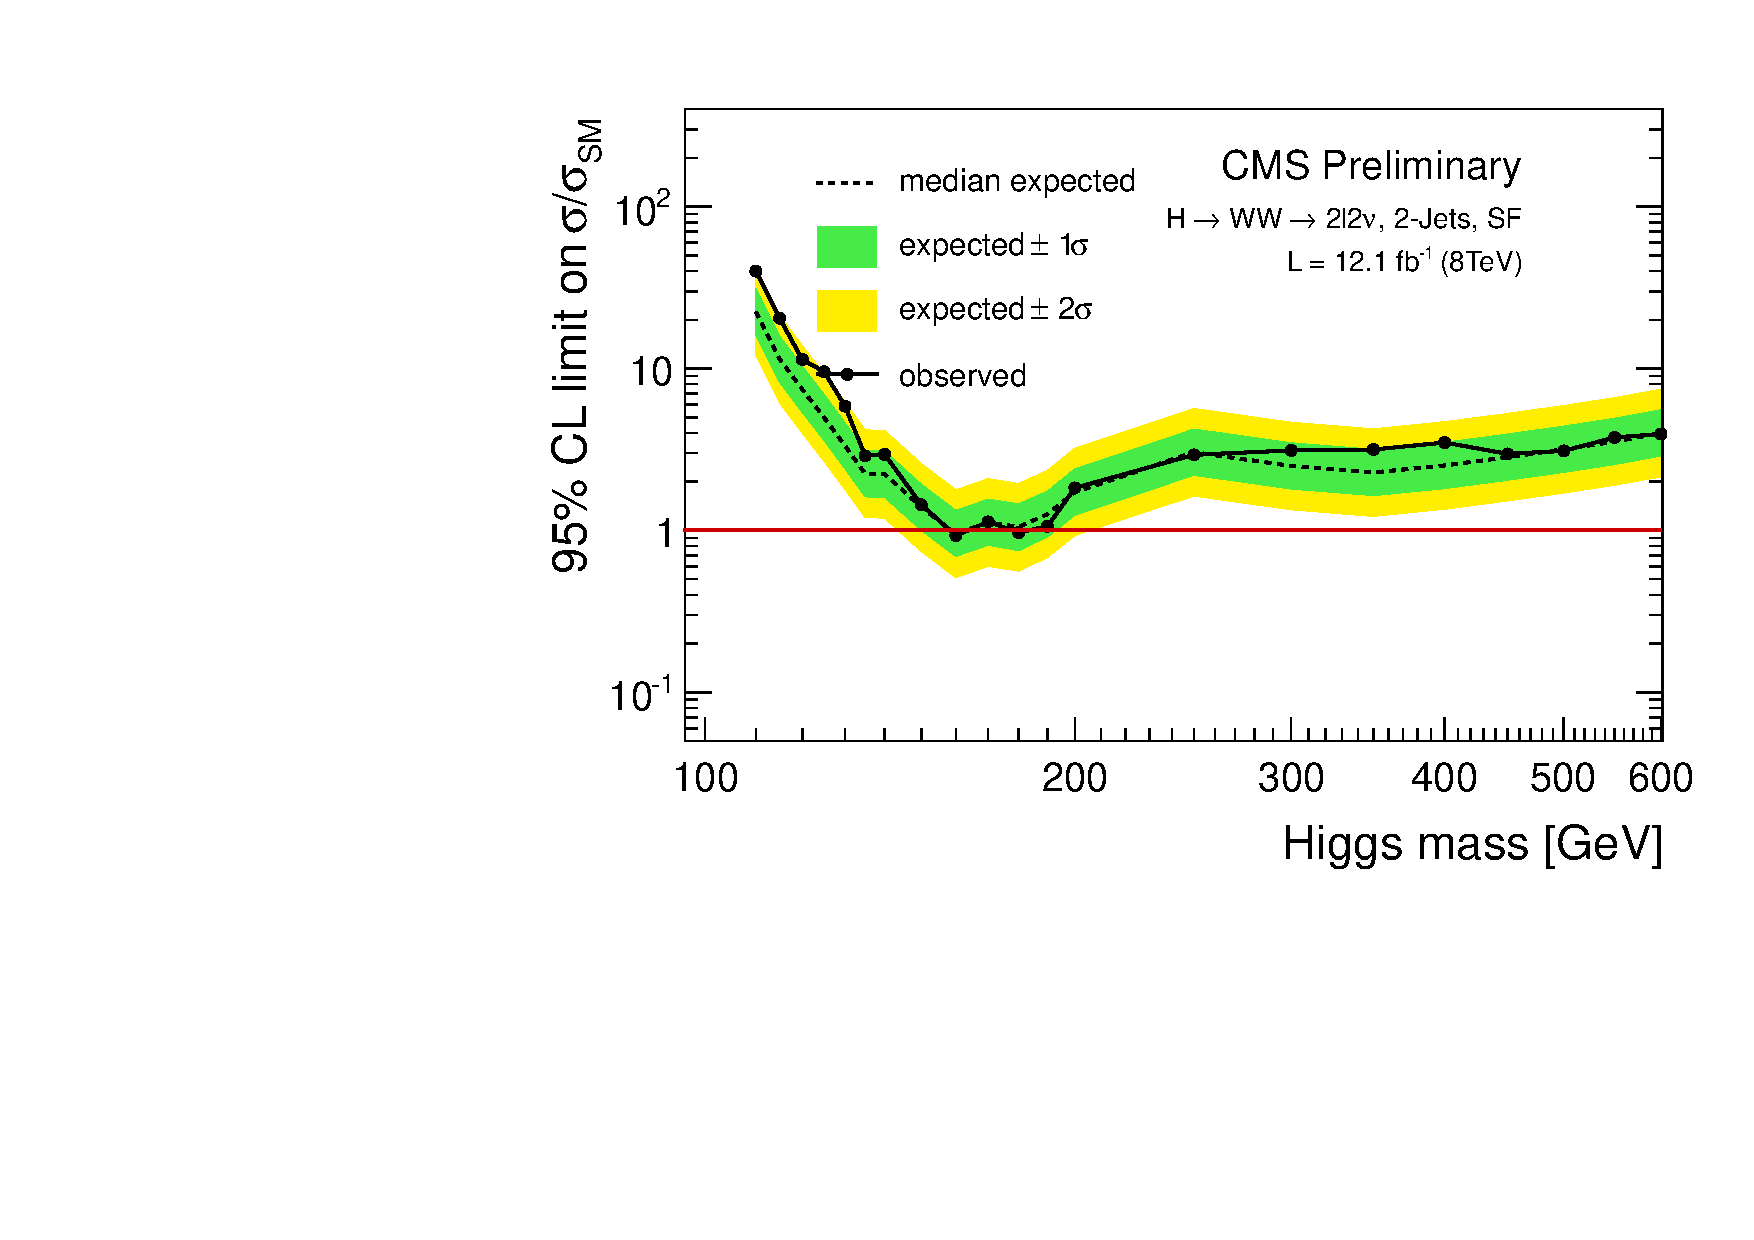
\includegraphics[width=.75\textwidth]{figures/table_limits_2j_cut_sf_log.pdf}
\caption{Expected upper limits for SM Higgs in $\intlumiEightTeV$ at 8 TeV with cut-based analysis in 2jet bin in sf final states.}
\label{fig:uls_cut_2j_sf}
\end{figure}
% table
\begin{table}[!htbp]
\begin{center}
\begin{tabular}{c c c c c}
\hline
\vspace{-3mm} && \\
Higgs Mass & Observed  & Median expected & Expected range for 68\% & Expected range for 95\%   \\
\hline
110 & 39.95 & 22.36 & [16.11, 31.11] & [12.00, 41.70] \\
115 & 20.45 & 11.43 & [8.23, 15.90] & [6.13, 21.32] \\
120 & 11.37 & 7.43 & [5.35, 10.34] & [3.99, 13.86] \\
125 & 9.56 & 4.98 & [3.59, 6.93] & [2.67, 9.29] \\
130 & 5.86 & 3.33 & [2.40, 4.63] & [1.79, 6.21] \\
135 & 2.89 & 2.24 & [1.61, 3.12] & [1.20, 4.18] \\
140 & 2.95 & 2.23 & [1.60, 3.10] & [1.19, 4.15] \\
150 & 1.44 & 1.39 & [1.00, 1.93] & [0.74, 2.59] \\
160 & 0.93 & 0.95 & [0.69, 1.33] & [0.51, 1.78] \\
170 & 1.13 & 1.12 & [0.81, 1.56] & [0.60, 2.09] \\
180 & 0.97 & 1.05 & [0.75, 1.46] & [0.56, 1.95] \\
190 & 1.06 & 1.26 & [0.91, 1.75] & [0.68, 2.35] \\
200 & 1.83 & 1.72 & [1.24, 2.40] & [0.93, 3.22] \\
250 & 2.93 & 3.04 & [2.19, 4.23] & [1.63, 5.67] \\
300 & 3.12 & 2.50 & [1.80, 3.48] & [1.34, 4.66] \\
350 & 3.16 & 2.28 & [1.64, 3.17] & [1.22, 4.24] \\
400 & 3.49 & 2.52 & [1.81, 3.50] & [1.35, 4.70] \\
450 & 2.97 & 2.83 & [2.04, 3.94] & [1.52, 5.28] \\
500 & 3.10 & 3.17 & [2.28, 4.41] & [1.70, 5.91] \\
550 & 3.75 & 3.54 & [2.55, 4.93] & [1.90, 6.61] \\
600 & 3.94 & 4.00 & [2.88, 5.56] & [2.14, 7.46] \\
\vspace{-3mm} && \\
\hline
\end{tabular}
\caption{Expected upper limits for SM Higgs in $\intlumiEightTeV$ at 8 TeV with cut-based analysis in 2jet bin in sf final states.}
\label{tab:uls_cut_2j_sf}
\end{center}
\end{table}
%%%%%%%%%%

\newpage
%%%%%%%%%%%%%%%%%
% plot
\begin{figure}[!hbtp]
\centering
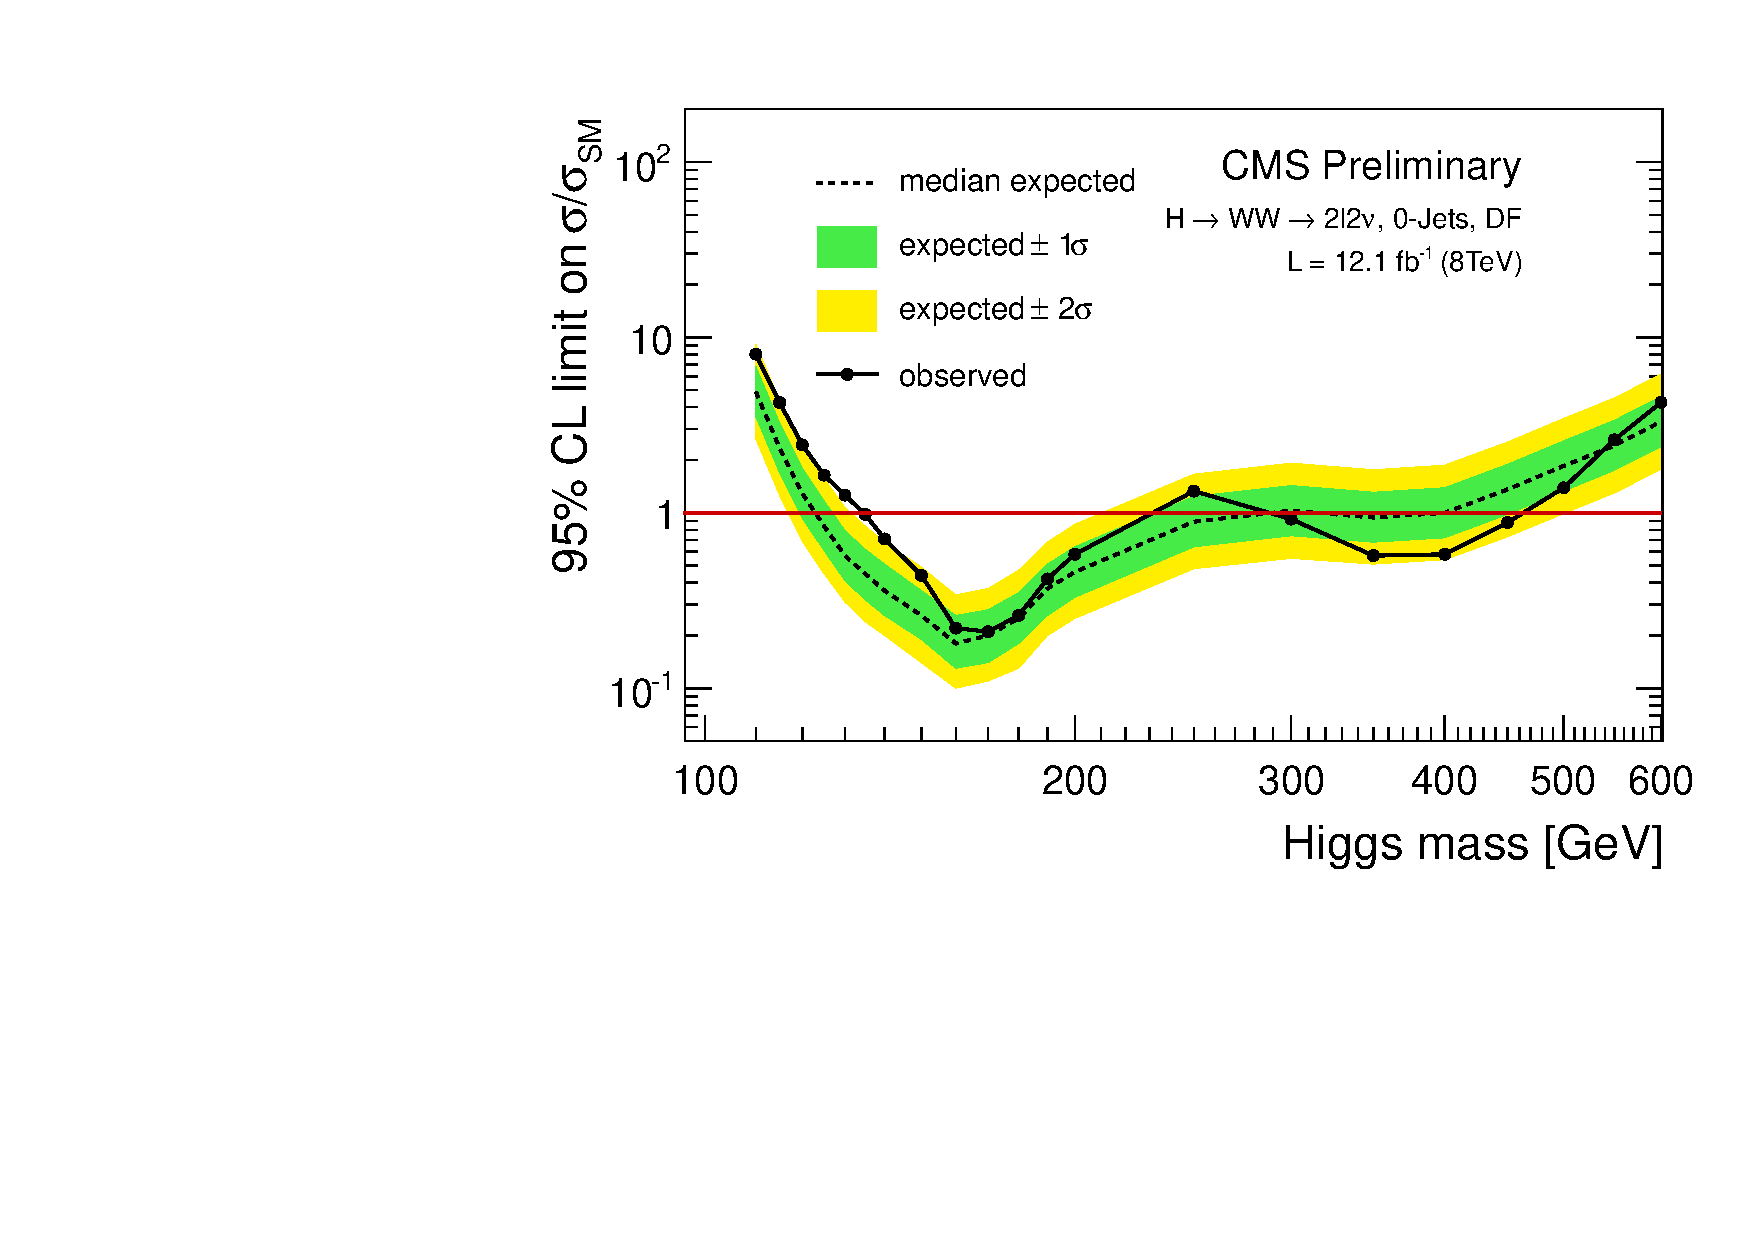
\includegraphics[width=.75\textwidth]{figures/table_limits_0j_shape_of_log.pdf} 
\caption{Expected upper limits for SM Higgs in $\intlumiEightTeV$ at 8 TeV with 2D analysis in 0jet bin in DF final states.}
\label{fig:uls_2d_0j_of}
\end{figure}
% table
\begin{table}[!htbp]
\begin{center}
\begin{tabular}{c c c c c}
\hline
\vspace{-3mm} && \\
Higgs Mass & Observed  & Median expected & Expected range for 68\% & Expected range for 95\%   \\
\hline
110 & 8.02 & 4.89 & [3.53, 6.81] & [2.63, 9.13] \\
115 & 4.25 & 2.34 & [1.69, 3.26] & [1.26, 4.37] \\
120 & 2.44 & 1.29 & [0.93, 1.80] & [0.69, 2.41] \\
125 & 1.64 & 0.84 & [0.61, 1.17] & [0.45, 1.57] \\
130 & 1.26 & 0.57 & [0.41, 0.79] & [0.31, 1.07] \\
135 & 0.98 & 0.45 & [0.32, 0.62] & [0.24, 0.84] \\
140 & 0.71 & 0.36 & [0.26, 0.51] & [0.20, 0.68] \\
150 & 0.44 & 0.26 & [0.19, 0.36] & [0.14, 0.49] \\
160 & 0.22 & 0.18 & [0.13, 0.26] & [0.10, 0.34] \\
170 & 0.21 & 0.20 & [0.14, 0.28] & [0.11, 0.37] \\
180 & 0.26 & 0.25 & [0.18, 0.35] & [0.13, 0.47] \\
190 & 0.42 & 0.37 & [0.26, 0.51] & [0.20, 0.68] \\
200 & 0.58 & 0.46 & [0.33, 0.64] & [0.25, 0.86] \\
250 & 1.33 & 0.89 & [0.64, 1.24] & [0.48, 1.66] \\
300 & 0.92 & 1.03 & [0.74, 1.43] & [0.55, 1.92] \\
350 & 0.57 & 0.94 & [0.68, 1.31] & [0.51, 1.76] \\
400 & 0.58 & 1.00 & [0.72, 1.39] & [0.54, 1.87] \\
450 & 0.88 & 1.36 & [0.98, 1.89] & [0.73, 2.53] \\
500 & 1.39 & 1.85 & [1.33, 2.57] & [0.99, 3.45] \\
550 & 2.61 & 2.42 & [1.75, 3.37] & [1.30, 4.52] \\
600 & 4.26 & 3.31 & [2.38, 4.60] & [1.77, 6.17] \\
\vspace{-3mm} && \\
\hline
\end{tabular}
\caption{Expected upper limits for SM Higgs in $\intlumiEightTeV$ at 8 TeV with 2D analysis in 0jet bin in DF final states.}
\label{tab:uls_2d_0j_of}
\end{center}
\end{table}
%%%%%%%%%%

%%%%%%%%%%%%%%%%%
% plot
\begin{figure}[!hbtp]
\centering
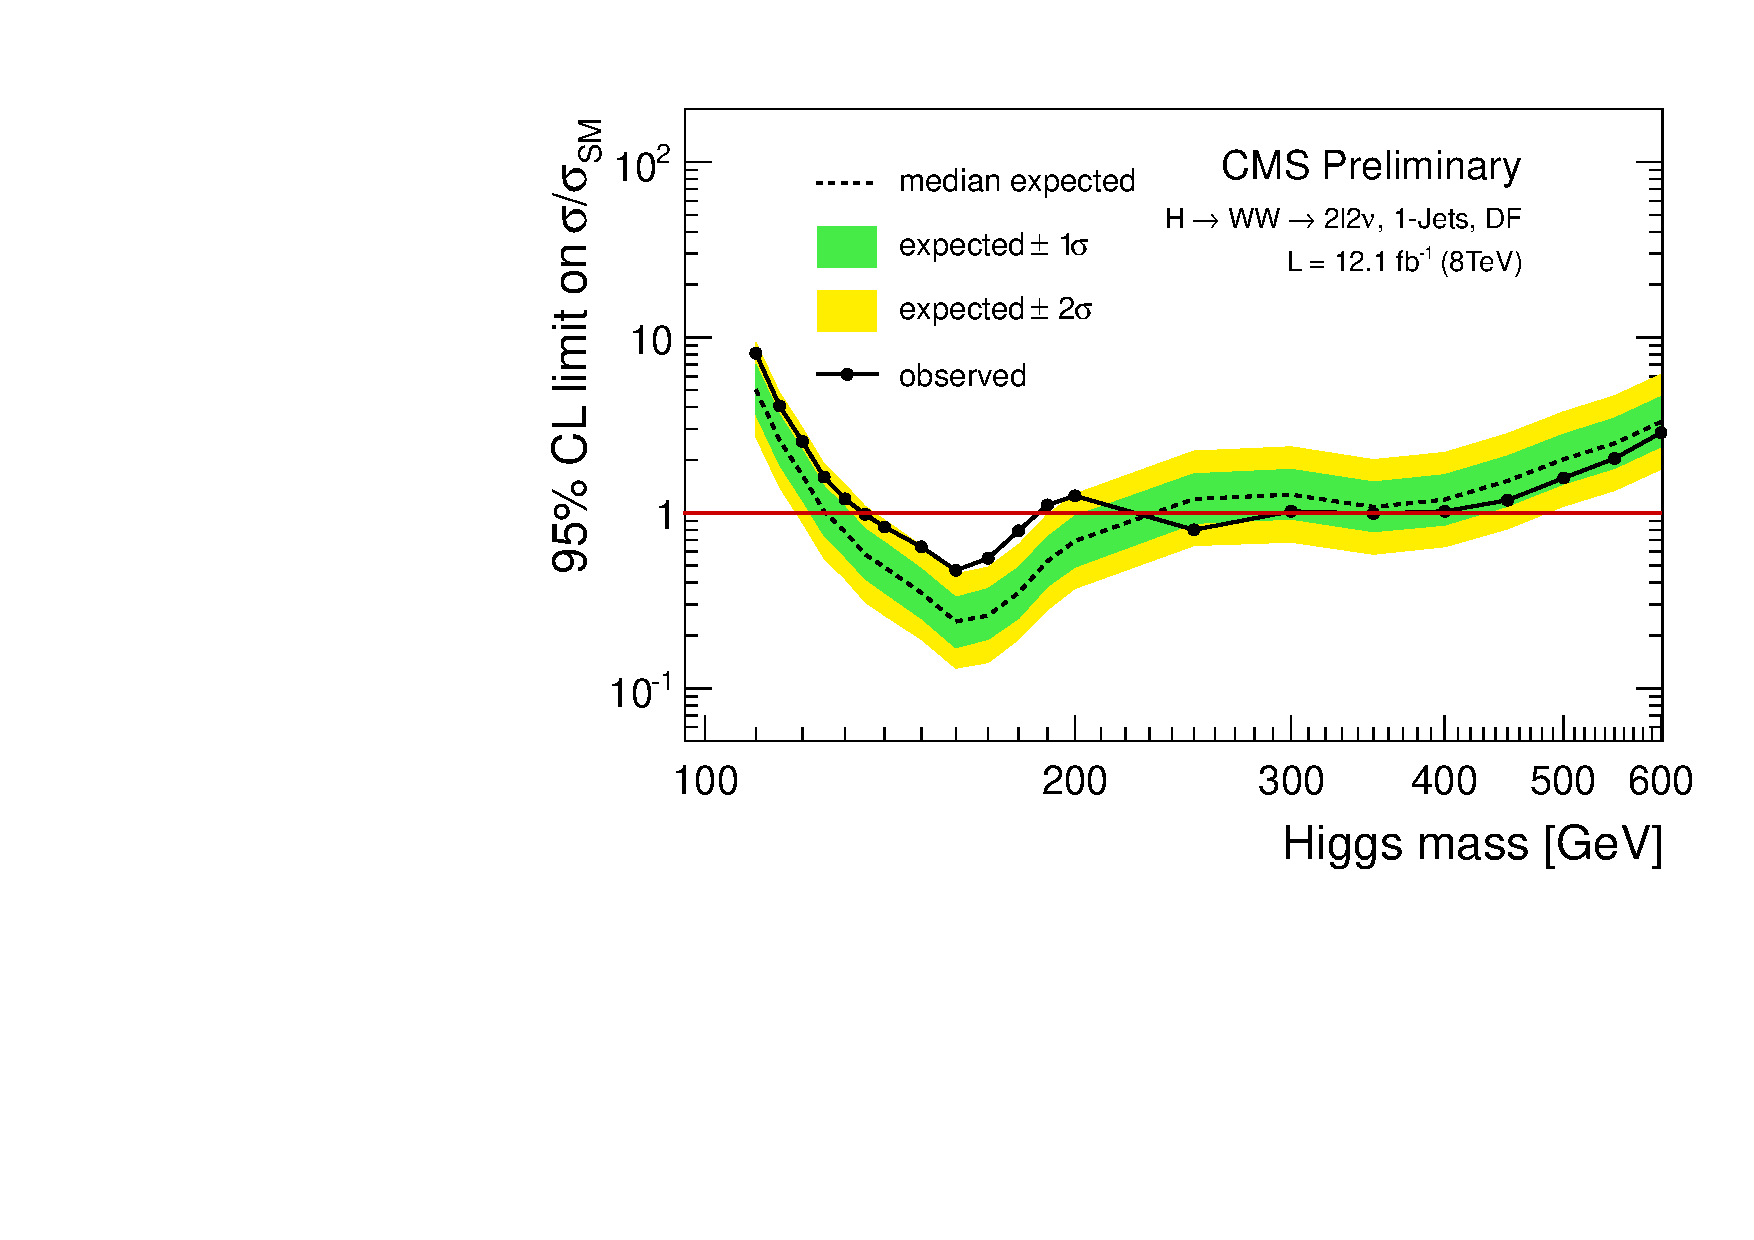
\includegraphics[width=.75\textwidth]{figures/table_limits_1j_shape_of_log.pdf}
\caption{Expected upper limits for SM Higgs in $\intlumiEightTeV$ at 8 TeV with 2D analysis in 1jet bin in DF final states.}
\label{fig:uls_2d_1j_of}
\end{figure}
% table
\begin{table}[!htbp]
\begin{center}
\begin{tabular}{c c c c c}
\hline
\vspace{-3mm} && \\
Higgs Mass & Observed  & Median expected & Expected range for 68\% & Expected range for 95\%   \\
\hline
110 & 8.12 & 5.04 & [3.63, 7.01] & [2.70, 9.40] \\
115 & 4.07 & 2.60 & [1.87, 3.62] & [1.40, 4.85] \\
120 & 2.55 & 1.64 & [1.18, 2.28] & [0.88, 3.06] \\
125 & 1.60 & 1.02 & [0.74, 1.42] & [0.55, 1.90] \\
130 & 1.20 & 0.78 & [0.56, 1.08] & [0.42, 1.45] \\
135 & 0.98 & 0.58 & [0.42, 0.81] & [0.31, 1.09] \\
140 & 0.83 & 0.49 & [0.35, 0.68] & [0.26, 0.91] \\
150 & 0.64 & 0.35 & [0.25, 0.48] & [0.19, 0.65] \\
160 & 0.47 & 0.24 & [0.17, 0.33] & [0.13, 0.45] \\
170 & 0.55 & 0.26 & [0.19, 0.37] & [0.14, 0.49] \\
180 & 0.79 & 0.35 & [0.25, 0.49] & [0.19, 0.66] \\
190 & 1.11 & 0.53 & [0.38, 0.73] & [0.28, 0.98] \\
200 & 1.25 & 0.69 & [0.49, 0.96] & [0.37, 1.28] \\
250 & 0.80 & 1.20 & [0.87, 1.67] & [0.65, 2.25] \\
300 & 1.02 & 1.27 & [0.92, 1.77] & [0.68, 2.38] \\
350 & 0.99 & 1.08 & [0.78, 1.50] & [0.58, 2.01] \\
400 & 1.02 & 1.19 & [0.85, 1.65] & [0.64, 2.21] \\
450 & 1.18 & 1.52 & [1.09, 2.11] & [0.81, 2.83] \\
500 & 1.58 & 2.02 & [1.46, 2.81] & [1.09, 3.77] \\
550 & 2.04 & 2.49 & [1.79, 3.47] & [1.34, 4.65] \\
600 & 2.86 & 3.30 & [2.38, 4.60] & [1.77, 6.16] \\
\vspace{-3mm} && \\
\hline
\end{tabular}
\caption{Expected upper limits for SM Higgs in $\intlumiEightTeV$ at 8 TeV with 2D analysis in 1jet bin in DF final states.}
\label{tab:uls_2d_1j_of}
\end{center}
\end{table}
%%%%%%%%%%





%%%%%%%%%%%%%%%%%%%%%%%%%%%%%%
%%%%%    Significance      %%%
%%%%%%%%%%%%%%%%%%%%%%%%%%%%%%
\newpage 
\begin{table}[!htbp]
\begin{center}
\begin{tabular}{c | c c}
\hline
\vspace{-3mm} && \\
Higgs Mass & Observed  & Expected \\
\hline \hline
\vspace{-3mm} && \\
115  & 0.9  & 0.6 \\
125  & 0.1  & 1.4 \\
140  & 0.0  & 2.5 \\
160  & 0.5  & 4.1 \\
200  & 0.0  & 2.3 \\
400  & 0.2  & 1.1 \\
600  & 0.0  & 0.8 \\
\hline
\end{tabular}
\caption{Observed and expected significances for SM Higgs in $\intlumiEightTeV$ at 8 TeV with cut-based analysis in 2jet bin in DF+SF final states.}
\label{tab:signif_cut_2j}
\end{center}
\end{table}

\begin{table}[!htbp]
\begin{center}
\begin{tabular}{c | c c}
\hline
\vspace{-3mm} && \\
Higgs Mass & Observed  & Expected \\
\hline \hline
\vspace{-3mm} && \\
115  & 2.2  & 1.1 \\
125  & 1.7  & 2.4 \\
140  & 1.8  & 4.8 \\
160  & 3.0  & 11.1 \\
200  & 2.0  & 4.4 \\
400  & 0.0  & 2.2 \\
600  & 0.0  & 1.2 \\
\hline
\end{tabular}
\caption{Observed and expected significances for SM Higgs in $\intlumiEightTeV$ at 8 TeV with cut-based analysis in 0/1/2jet bins in DF+SF final states.}
\label{tab:signif_cut}
\end{center}
\end{table}

\begin{table}[!htbp]
\begin{center}
\begin{tabular}{c | c c}
\hline
\vspace{-3mm} && \\
Higgs Mass & Observed  & Expected \\
\hline \hline
\vspace{-3mm} && \\
115  & 2.9  & 1.4 \\
125  & 2.0  & 3.4 \\
140  & 3.0  & 7.7 \\
160  & 3.1  & 19.0 \\
200  & 3.4  & 6.6 \\
400  & 0.0  & 3.5 \\
600  & 0.0  & 1.8 \\
\hline 
\end{tabular}
\caption{Observed and expected significances for SM Higgs in $\intlumiEightTeV$ at 8 TeV with BDT analysis in DF 0/1jet bins and cut-based analysis in other channels.}
\label{tab:signif_bdt01_cut2_cutsf}
\end{center}
\end{table}


\begin{table}[!htbp]
\begin{center}
\begin{tabular}{c | c c}
\hline
\vspace{-3mm} && \\
Higgs Mass & Observed  & Expected \\
\hline \hline
\vspace{-3mm} && \\
115  & 3.0  & 1.5 \\
125  & 2.8  & 3.7 \\
140  & 3.2  & 7.8 \\
160  & 3.1  & 16.6 \\
200  & 1.6  & 6.1 \\
400  & 0.0  & 3.3 \\
600  & 0.0  & 1.5 \\
\hline
\end{tabular}
\caption{Observed and expected significances for SM Higgs in $\intlumiEightTeV$ at 8 TeV with 2D analysis in DF 0/1jet bins and cut-based analysis in other channels.}
\label{tab:signif_2d01_cut2_cutsf}
\end{center}
\end{table}


%%% individual channels 
\newpage 
\begin{table}[!htbp]
\begin{center}
\begin{tabular}{c | c c}
\hline
\vspace{-3mm} && \\
Higgs Mass & Observed  & Expected \\
\hline \hline
\vspace{-3mm} && \\ 
115  & 1.6  & 0.8 \\
125  & 1.7  & 1.7 \\
140  & 1.7  & 3.7 \\
160  & 2.4  & 9.4 \\
200  & 2.2  & 3.2 \\
400  & 0.0  & 1.6 \\
600  & 0.0  & 0.6 \\
\hline
\end{tabular}
\caption{Observed and expected significances for SM Higgs in $\intlumiEightTeV$ at 8 TeV with cut-based analysis in 0jet bin in DF final states.}
\label{tab:signif_cut_0j_of}
\end{center}
\end{table}

\begin{table}[!htbp]
\begin{center}
\begin{tabular}{c | c c}
\hline
\vspace{-3mm} && \\
Higgs Mass & Observed  & Expected \\
\hline \hline
\vspace{-3mm} && \\
115  & 1.6  & 0.7 \\
125  & 1.5  & 1.6 \\
140  & 1.6  & 3.2 \\
160  & 2.3  & 6.9 \\
200  & 2.5  & 2.5 \\
400  & 0.0  & 1.3 \\
600  & 0.0  & 0.6 \\
\hline
\end{tabular}
\caption{Observed and expected significances for SM Higgs in $\intlumiEightTeV$ at 8 TeV with cut-based analysis in 1jet bin in DF final states.}
\label{tab:signif_cut_1j_of}
\end{center}
\end{table}

\begin{table}[!htbp]
\begin{center}
\begin{tabular}{c | c c}
\hline
\vspace{-3mm} && \\
Higgs Mass & Observed  & Expected \\
\hline \hline
\vspace{-3mm} && \\
115  & 0.2  & 0.6 \\
125  & 0.0  & 1.3 \\
140  & 0.0  & 2.3 \\
160  & 0.6  & 3.9 \\
200  & 0.0  & 2.1 \\
400  & 0.0  & 0.9 \\
600  & 0.0  & 0.6 \\
\hline
\end{tabular}
\caption{Observed and expected significances for SM Higgs in $\intlumiEightTeV$ at 8 TeV with cut-based analysis in 2jet bin in DF final states.}
\label{tab:signif_cut_2j_of}
\end{center}
\end{table}

\newpage 
\begin{table}[!htbp]
\begin{center}
\begin{tabular}{c | c c}
\hline
\vspace{-3mm} && \\
Higgs Mass & Observed  & Expected \\
\hline \hline
\vspace{-3mm} && \\
115  & 1.4  & 0.5 \\
125  & 0.9  & 1.3 \\
140  & 1.2  & 2.8 \\
160  & 1.8  & 6.4 \\
200  & 1.2  & 3.0 \\
400  & 0.0  & 1.1 \\
600  & 0.0  & 0.6 \\
\hline
\end{tabular}
\caption{Observed and expected significances for SM Higgs in $\intlumiEightTeV$ at 8 TeV with cut-based analysis in 0jet bin in SF final states.}
\label{tab:signif_cut_0j_sf}
\end{center}
\end{table}

\begin{table}[!htbp]
\begin{center}
\begin{tabular}{c | c c}
\hline
\vspace{-3mm} && \\
Higgs Mass & Observed  & Expected \\
\hline \hline
\vspace{-3mm} && \\
115  & 1.5  & 0.4 \\
125  & 1.7  & 1.1 \\
140  & 2.1  & 2.5 \\
160  & 1.0  & 5.4 \\
200  & 0.8  & 2.1 \\
400  & 0.0  & 1.1 \\
600  & 0.0  & 0.6 \\
\hline
\end{tabular}
\caption{Observed and expected significances for SM Higgs in $\intlumiEightTeV$ at 8 TeV with cut-based analysis in 1jet bin in SF final states.}
\label{tab:signif_cut_1j_sf}
\end{center}
\end{table}

\begin{table}[!htbp]
\begin{center}
\begin{tabular}{c | c c}
\hline
\vspace{-3mm} && \\
Higgs Mass & Observed  & Expected \\
\hline \hline
\vspace{-3mm} && \\
115  & 1.8  & 0.3 \\
125  & 2.1  & 0.6 \\
140  & 0.9  & 1.0 \\
160  & 0.0  & 1.4 \\
200  & 0.2  & 1.1 \\
400  & 0.9  & 0.9 \\
600  & 0.0  & 0.7 \\
\hline
\end{tabular}
\caption{Observed and expected significances for SM Higgs in $\intlumiEightTeV$ at 8 TeV with cut-based analysis in 2jet bin in SF final states.}
\label{tab:signif_cut_2j_sf}
\end{center}
\end{table}

\newpage 
\begin{table}[!htbp]
\begin{center}
\begin{tabular}{c | c c}
\hline
\vspace{-3mm} && \\
Higgs Mass & Observed  & Expected \\
\hline \hline
\vspace{-3mm} && \\
115  & 1.7  & 0.9 \\
125  & 2.1  & 2.5 \\
140  & 2.1  & 5.6 \\
160  & 1.0  & 12.3 \\
200  & 0.6  & 4.4 \\
400  & 0.0  & 2.0 \\
600  & 1.0  & 0.6 \\
\hline
\end{tabular}
\caption{Observed and expected significances for SM Higgs in $\intlumiEightTeV$ at 8 TeV with 2D analysis in 0jet bin in DF final states.}
\label{tab:signif_2d_0j_of}
\end{center}
\end{table}

\begin{table}[!htbp]
\begin{center}
\begin{tabular}{c | c c}
\hline
\vspace{-3mm} && \\
Higgs Mass & Observed  & Expected \\
\hline \hline
\vspace{-3mm} && \\
115  & 1.2  & 0.9 \\
125  & 1.2  & 2.1 \\
140  & 1.4  & 4.3 \\
160  & 2.3  & 9.3 \\
200  & 1.9  & 3.0 \\
400  & 0.0  & 1.8 \\
600  & 0.0  & 0.8 \\
\hline
\end{tabular}
\caption{Observed and expected significances for SM Higgs in $\intlumiEightTeV$ at 8 TeV with 2D analysis in 1jet bin in DF final states.}
\label{tab:signif_2d_1j_of}
\end{center}
\end{table}



%%%%%%%%%%%%%%%%%%%%%%%%%%%%%%%%%%%%%%%%%%%%%%%%%%%%%%%%%%%%%%%%%%%%
%%%%%  THESE NEED TO BE MOVED TO APPROPRIATE PLACES
%%%%%%%%%%%%%%%%%%%%%%%%%%%%%%%%%%%%%%%%%%%%%%%%%%%%%%%%%%%%%%%%%%%%

\begin{table}[!htbp]
\begin{center}
\begin{tabular}{c | c c | c c  }
\hline \hline 
\vspace{-3mm} && \\
Higgs Mass(\GeV) & \multicolumn{2}{c}{BDT 0/1j OF + cut VBF OF} & \multicolumn{2}{c}{2D 0/1j OF+ cut VBF OF} \\
\hline 
				 & Observed  & Expected 					 	& Observed  & Expected  \\
\hline \hline
115 & 2.0  	& 1.2 	& 2.2 & 1.4 \\
125 & 1.1  	& 3.0  	& 2.2 & 3.4 \\
140 & 2.2  	& 6.8 	& 2.5 & 7.2 \\
160 & 2.5 	& 17.4  & 2.5 & 15.1 \\
200 & 3.1 	& 6.1  	& 1.3 & 5.6 \\
400 & 0 	& 3.2 	& 0   & 2.9 \\
600 & 0  	& 1.5 	& 0   & 1.1 \\
\hline \hline
\end{tabular}
\caption{Expected and observed significances SM Higgs in $\intlumiEightTeV$ at 8 TeV in DF final states.}
\label{tab:significance_8TeV}
\end{center}
\end{table} 

